%Introductory sentences here
In this section, we describe how we generated a realistic simulated data set for dexterous grasping. This captures variations in both observable (e.g. object pose) and unobservable (e.g. surface friction) parameters.

To generate the training set a simulated depth image of a scene containing a single unfamiliar object is generated. Using either of the generative models GM1 or GM2, grasps are generated and executed in simulation. The success or failure of each simulated grasp is recorded. Producing a good simulation for evaluating grasps is non-trivial. An important problem is that the data set must capture the natural uncertainty in unobservable variables, such as mass and friction. Since many of these parameters are unobservable we are thus creating a data set such that the grasp policy must work across a range of variations. This is thus a form of {\em domain randomisation}. A similar technique has been employed by \cite{mahler2017dex}, but we extend it from a single grasp quality metric to full rigid body simulation.

\subsection{Features and Constraints of the Virtual Environment}
\label{subsection:environment}

The collected 3D model dataset contains 294 objects from 20 classes, namely, bottles, bowls, cans, boxes, cups, mugs, pans, salt and pepper shakers, plates, forks, spoons, spatulas, knives, teapots, teacups, tennis balls, dustpans, scissors, funnels and jugs (Figure \ref{fig:allObjects}). All objects in the dataset can be grasped using the DLR-II hand, although there are limitations on how some object classes can be approached. For example, teapots and jugs are not easy to grasp except by their handles due being larger than the hand's maximum aperture, while small objects such as salt and pepper shakers can be approached in more creative ways. The number of objects in each class varies from 1 (dustpan) to 25 (bottles). Long/thin objects such as kitchen utensils are placed vertically in a short, heavy stand in order to make them graspable without touching the table. This reflects the real-world scenario, as attempting to grasp a spatula lying on a table would be dangerous for the robotic hand. In total, 250 objects from all 20 classes were allocated for training and validation, while the remaining 44 objects from 19 classes belong to the test set.

We employ MuJoCo \cite{MuJoCo} as the rigid-body simulator. Due to the fact that collision checking in MuJoCo requires that objects comprise convex parts, all 294 objects were decomposed into convex parts using V-HACD algorithm \cite{V-HACD}. The number of sub-parts varies from 2 to 120.

During the scene creation, the object is placed on the virtual table at a pseudo-random pose. Most objects are placed in a canonical upright pose, and only randomly rotated around the gravity axis (akin to being placed on a turntable). The objects belonging to the mug and cup classes have fully random 3D rotations applied before they are placed on the table, since it is possible to grasp them in almost any setting using the robot hand.

\begin{figure}
  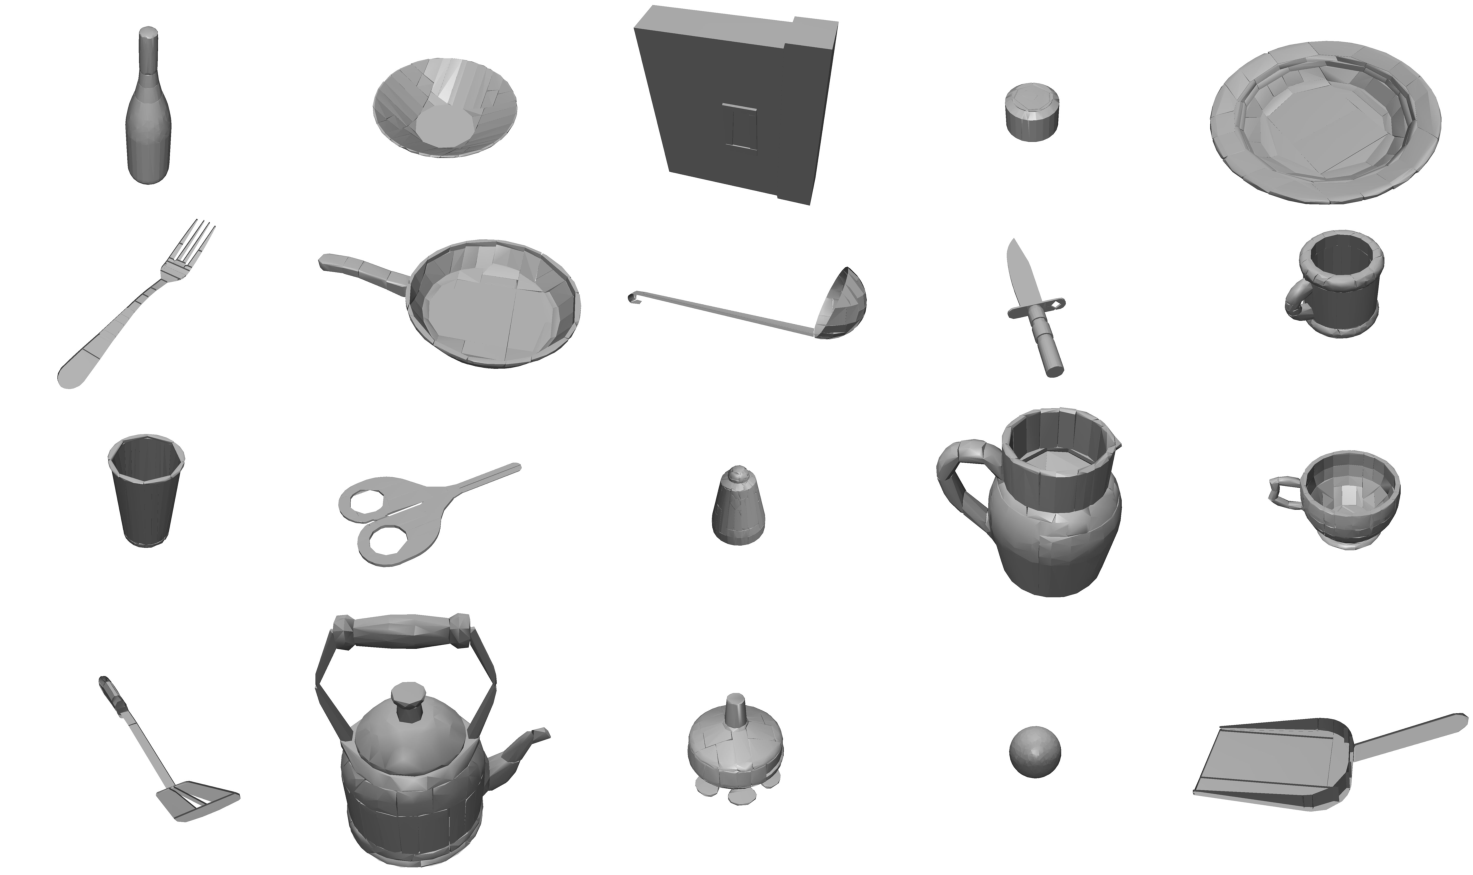
\includegraphics[width=\linewidth]{images/allObjects-small.pdf}
  \caption{A sample of the 294 objects drawn from the 20 object classes.
  \label{fig:allObjects}}
\end{figure}

To achieve domain randomisation, prior distributions for mass, size and frictional coefficient were estimated from real-world data. The properties of simulated objects are sampled from these priors. For each object its mean size, mass and friction coefficient are matched to a real counterpart. For each trial, the size is randomly scaled by a factor in the range [0.9,1.1], while remaining within the grasp aperture of the hand. Object mass is uniformly sampled from a category specific range, estimated from real objects (Table~\ref{fig:weights}). The friction coefficient of each object is sampled from a range of $[0.5, 1]$ in MuJoCo default units, intended to simulate surfaces from low-friction (metal) to high-friction (rubber). This variation is critical to ensuring that the evaluative model will predict the robustness of a grasp to unobservable variations.
\begin{table}[]
\centering
\caption{Mass ranges for each object class (grams).}
\label{fig:weights}
\resizebox{\linewidth}{!}{\begin{tabular}{|l|l|l|l|l|l|l|}
\hline
Bottle & Bowl     & Box     & Can     & Cup    & Fork    & Pan     \\ \hline
30-70  & 50-400   & 50-500  & 200-400 & 30-330 & 40-80   & 150-450 \\ \hline
Plate  & Scissors & Shaker  & Spatula & Spoon  & Teacup  & Teapot  \\ \hline
40-80  & 50-150   & 100-160 & 40-80   & 40-80  & 150-250 & 500-800 \\ \hline
Jug    & Knife    & Mug     & Funnel  & Ball   & Dustpan &         \\ \hline
80-200 & 50-150   & 250-350 & 40-80   & 50-70  & 100-150 &         \\ \hline
\end{tabular}}
\end{table}
 
For depth image simulation the Carmine 1.09 depth sensor installed on the robot is simulated with a modified version of the Blensor Kinect sensor simulator \cite{KinectSimulator}. For each object, we vary the camera orientation and distance from the object, as well as object mass, friction, scale, location and orientation. In order to account for calibration errors in the real world setup, we add a small three-dimensional positional noise to each point in the sensor output.

A 3D mesh-model of the DLR-II hand has been used in the simulator. There are no kinematic constraints on how the hand may grasp an object, other than collisions with the table. To ensure realism, we use impedance control for the hand.
%The reasons for the most critical of these decisions are now given in slightly more detail. First, in order to create a realistic simulation environment, we chose the MuJoCo \cite{MuJoCo} physics simulator over other simulators (OpenSim, BulletPhysics, ODE, NVIDIA PhysX) for two reasons: 
%\begin{itemize}
%\item MuJoCo uses generalized coordinates and optimization-based contact dynamics, resulting in fewer numerical instabilities,
%\item MuJoCo is optimized for the quality of physics as well as its speed, hence improving the quality of the physics simulation.
%\end{itemize}
\begin{figure}
  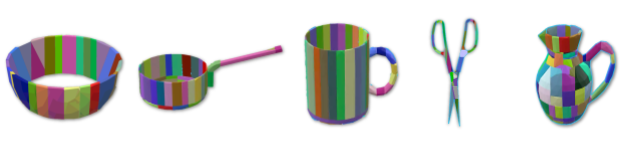
\includegraphics[width=\linewidth]{images/decomposition.png}
  \caption{Approximate convex decomposition of some objects in our dataset. Best viewed in colour.}
  \label{fig:objectDecomposition}
\end{figure}

Some classes are easier to grasp than others. Table \ref{fig:graspperf} shows the success rates of the generated grasps in each class, when attempted with the grasps ranked by the Generative Model (GM1). The sampled grasps perform well on a number of classes including Dustpans, Scissors, Spoons, and Mugs. Some objects can only be grasped in certain ways, i.e. not all 10 training grasps are applicable to all objects.

\begin{table}[]
\centering
\caption{The average and \textbf{top} grasp success rates (\%) of GM1 on simulated data.}
\label{fig:graspperf}
\resizebox{\linewidth}{!}{\begin{tabular}{|l|l|l|l|l|l|l|}
\hline
Bottle & Bowl     & Box     & Can     & Cup    & Fork    & Pan     \\ \hline
35 - \textbf{47} & 26 - \textbf{61}   & 16 - \textbf{30}  & 41 - \textbf{92} & 44 - \textbf{59} & 59 - \textbf{68}   & 37 - \textbf{57} \\ \hline
Plate  & Scissors & Shaker  & Spatula & Spoon  & Teacup  & Teapot  \\ \hline
50 - \textbf{95}  & 62 - \textbf{69}   & 47 - \textbf{53} & 57 - \textbf{65}   & 63 - \textbf{82}  & 48 - \textbf{91} & 26 - \textbf{23} \\ \hline
Jug    & Knife    & Mug     & Funnel  & Ball   & Dustpan &         \\ \hline
24 - \textbf{43} & 58 - \textbf{65}   & 40 - \textbf{80} & 52 - \textbf{65}   & 28 - \textbf{82}  & 60 - \textbf{78} & 45 - \textbf{63} \\ \hline
\end{tabular}}
\end{table}

%\begin{table}[]
%\centering
%\caption{Mass ranges for each object class (grams).}
%\label{fig:weights}
%\resizebox{\linewidth}{!}{\begin{tabular}{|l|l|l|l|l|l|l|}
%\hline
%Bottle & Bowl     & Box     & Can     & Cup    & Fork    & Pan     \\ \hline
%35.5 - \textbf{47.7}\% & 26.4 - \textbf{61.2}\%   & 16.5 - \textbf{30.1}\%  & 41.4 - \textbf{92.6}\% & 44.7 - \textbf{59.9}\% & 59.6 - \textbf{68.1}\%   & 37.9 - %\textbf{57.3}\% \\ \hline
%Plate  & Scissors & Shaker  & Spatula & Spoon  & Teacup  & Teapot  \\ \hline
%50.2 - \textbf{95.5}\%  & 62.7 - \textbf{69.9}\%   & 47.3 - \textbf{53.3}\% & 57.4 - \textbf{65.7}\%   & 63.4 - \textbf{82.4}\%  & 48.2 - \textbf{91.2}\% & 26.9 - %\textbf{23.9}\% \\ \hline
%Jug    & Knife    & Mug     & Funnel  & Ball   & Dustpan &         \\ \hline
%24.9 - \textbf{43.9}\% & 58.3 - \textbf{65.0}\%   & 40.7 - \textbf{80.9}\% & 52.3 - \textbf{65.9}\%   & 28.0 - \textbf{82.8}\%  & 60.1 - \textbf{78.8}\% & 45.8 - %\textbf{63.2}\%        \\ \hline
%\end{tabular}}
%\end{table}

\subsection{Data Collection Methodology}
\label{subsection:dataCollection}

The data set is divided into units called \textit{scenes}, where each scene comprises a single object placed on a table. This object has a specific set of physical parameters, chosen as described below. Many views and grasps are attempted per scene. Below, we specify the time flow of data collection:

\begin{enumerate}
\item A novel instance of an object from the dataset is generated and placed on a virtual table. Variations are applied to object pose, scale, mass, and friction coefficients.
\item A simulated camera takes a depth image $I_s$ of the scene, converted to a point cloud $P_s$. The viewpoint ${elevation}_s$ of the view point is from 30-57 degrees. The ${azimuth}_s$ is sampled from $[0, 2\pi]$. 
\item The positions of all points in the point cloud $P_s$ are shifted by a three-dimensional noise vector sampled from a Gaussian distribution with parameters $\mu=0$ and $\sigma = 0.004$ (unit: meter).
\item Given $P_s$, the chosen generative model (GM1 or GM2) proposes the candidate grasps. For GM1, up to100 grasps are selected. These are the 10 grasps that are highest ranked by the GM for each of the 10 training grasps. For GM2, we select a maximum of 500 grasps: up to 50 grasps from each training grasp.
\item The grasps are applied to the object in simulation. Before the execution of each grasp, we run a collision check with the virtual table (without the object). If any part of the hand touches the table during this test, the grasp is marked as \textit{collided}, and not executed.
\item 19 further simulated depth images are taken from other viewpoints around the object, as explained in step 2. Images with fewer than 250 depth points are discarded. We then sample with replacement from the remaining images and associate each sampled image and viewpoint with a grasp created in step 3.
\item The grasp outcome, trajectory and depth image are stored for each trial. The grasp parameters are converted to the camera frame for the associated view.
\end{enumerate}

%Each candidate grasp $h_i = \{w_0, ..., w_{n}\}$ consists of a series of 10 waypoints along : $w_0$, ..., $w_{n}$. A waypoint $w_k$ is a 27-element vector that specifies full configuration of the hand in joint space: 3 dimensions for 3D coordinates and 4 dimensions for the orientation of the wrist, and 20 parameters specifying each finger joint's activation. 
%After a grasp $h_i$ is generated in world coordinates, the waypoints that belong to the grasp are converted to the camera's frame of reference. 
%The goal of our network architecture is to learn which grasps are more likely to succeed given a point cloud, where both input channels are represented in terms of the camera frame of reference. %This point differentiates us from the work of Levine et al. \cite{Levine1}, where camera coordinates are not used. It should be noted that the possible camera locations in our simulated data covers a larger space, with full circular movement $[0, 2\pi]$ on azimuth and $[30-57]$ range in elevation. Our scenes do not have any distinguishing landmarks such as a bin or robot base, which may aid the network in locating the camera in the scene. 

In each scene $S_i$, a number of depth images are taken $\{I_{ik}\}_{k=0}^{20}$, in the manner explained above. The first image $I_{i0}$ is used to generate grasps, as explained in Section \ref{section:generative}. We typically perform 10-500 grasps per scene. Attaching different views to each grasp instead of the seed image $I_{i0}$ ensures there is more variation in terms of viewpoints, resulting in a richer dataset. Typically, performing a grasp takes half the time it takes to acquire an image using the simulated camera.

Once a grasp is performed in simulation, it is considered a success if an object is lifted one metre above the table, and held there for two seconds. If the object slips from the hand during lifting or holding, the grasp is a failure. 

\begin{figure}[t]
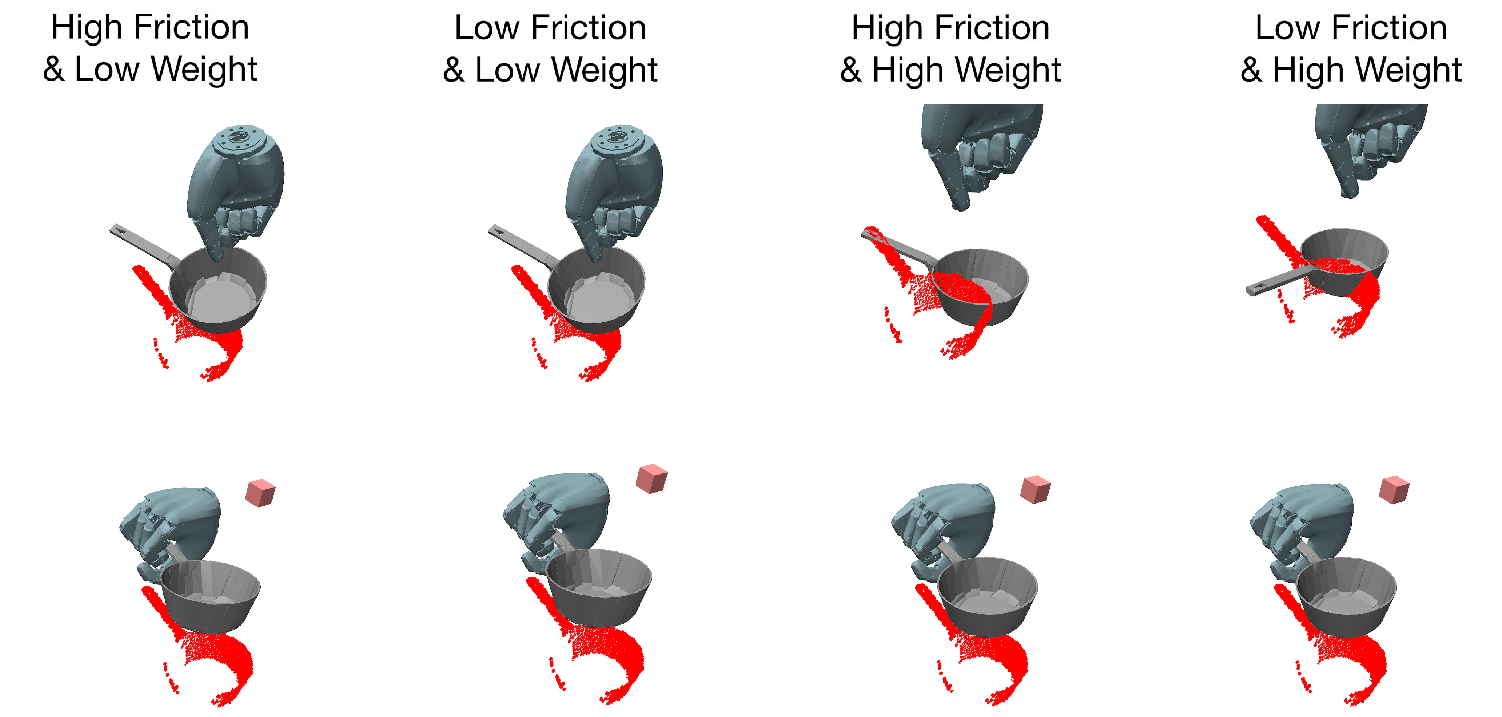
\includegraphics[width=\columnwidth]{images/frictionweight}
%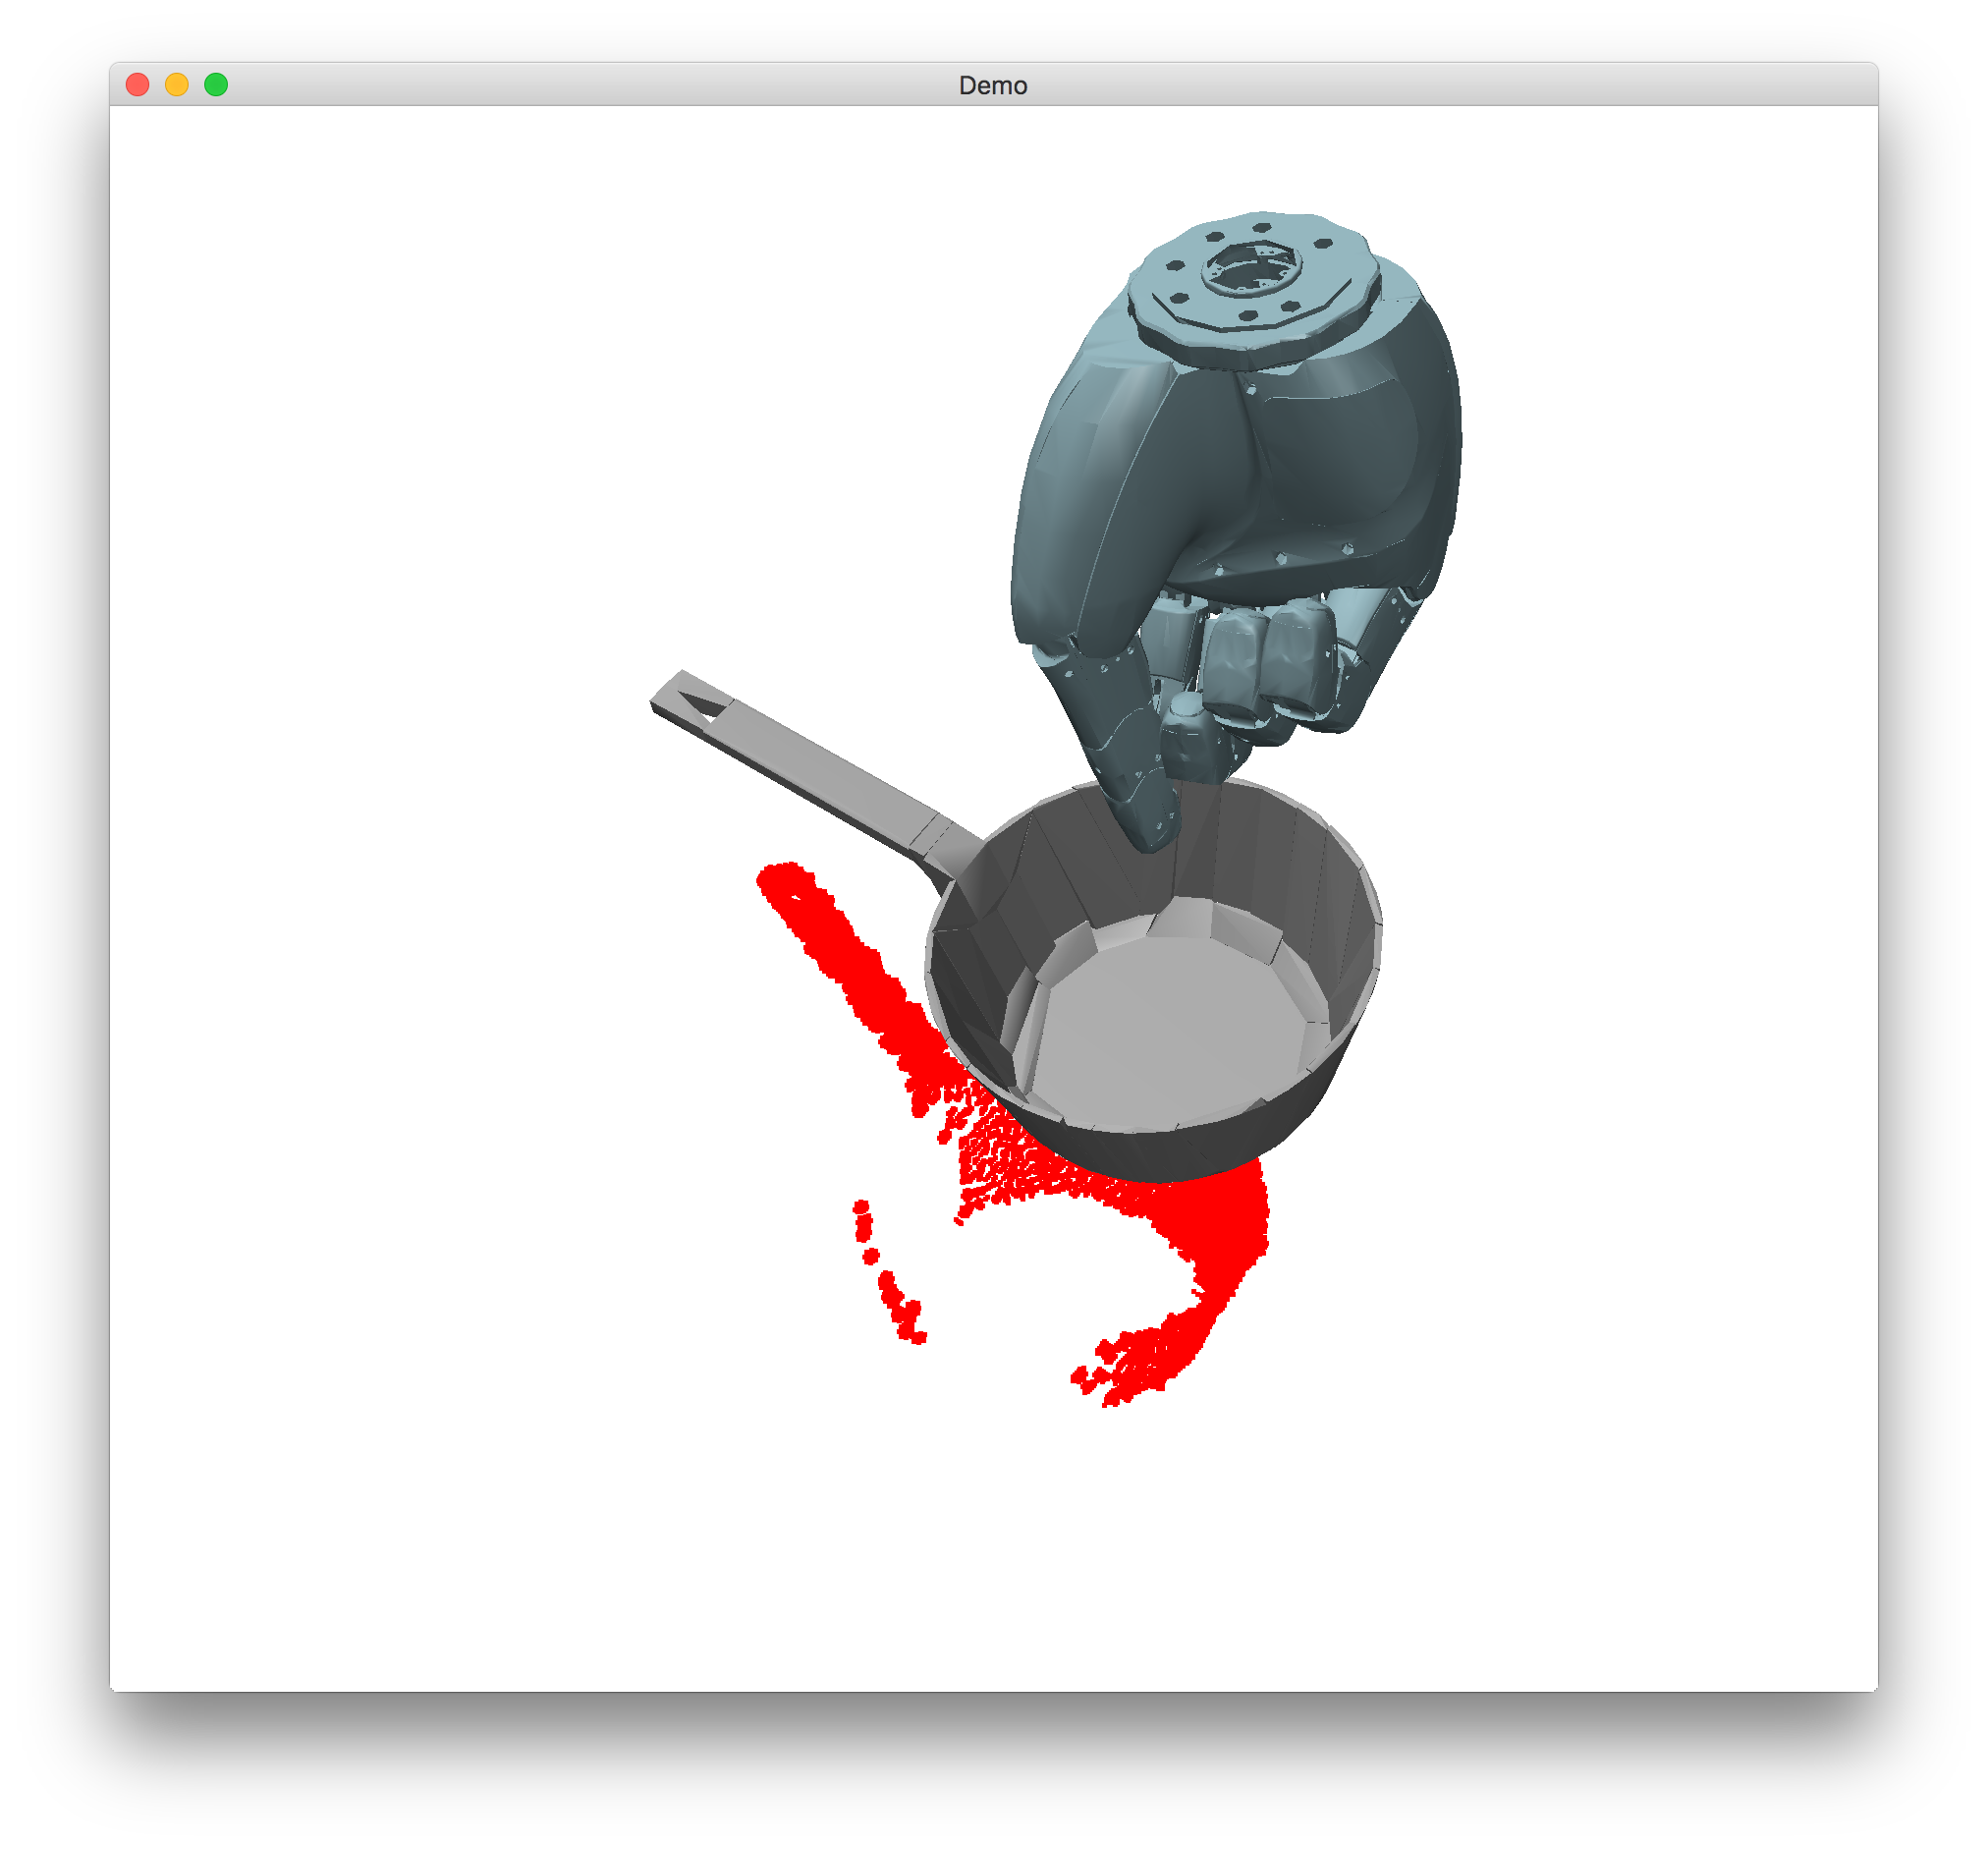
\includegraphics[width=0.24\textwidth]{images/Pan4_2_HFLW}
%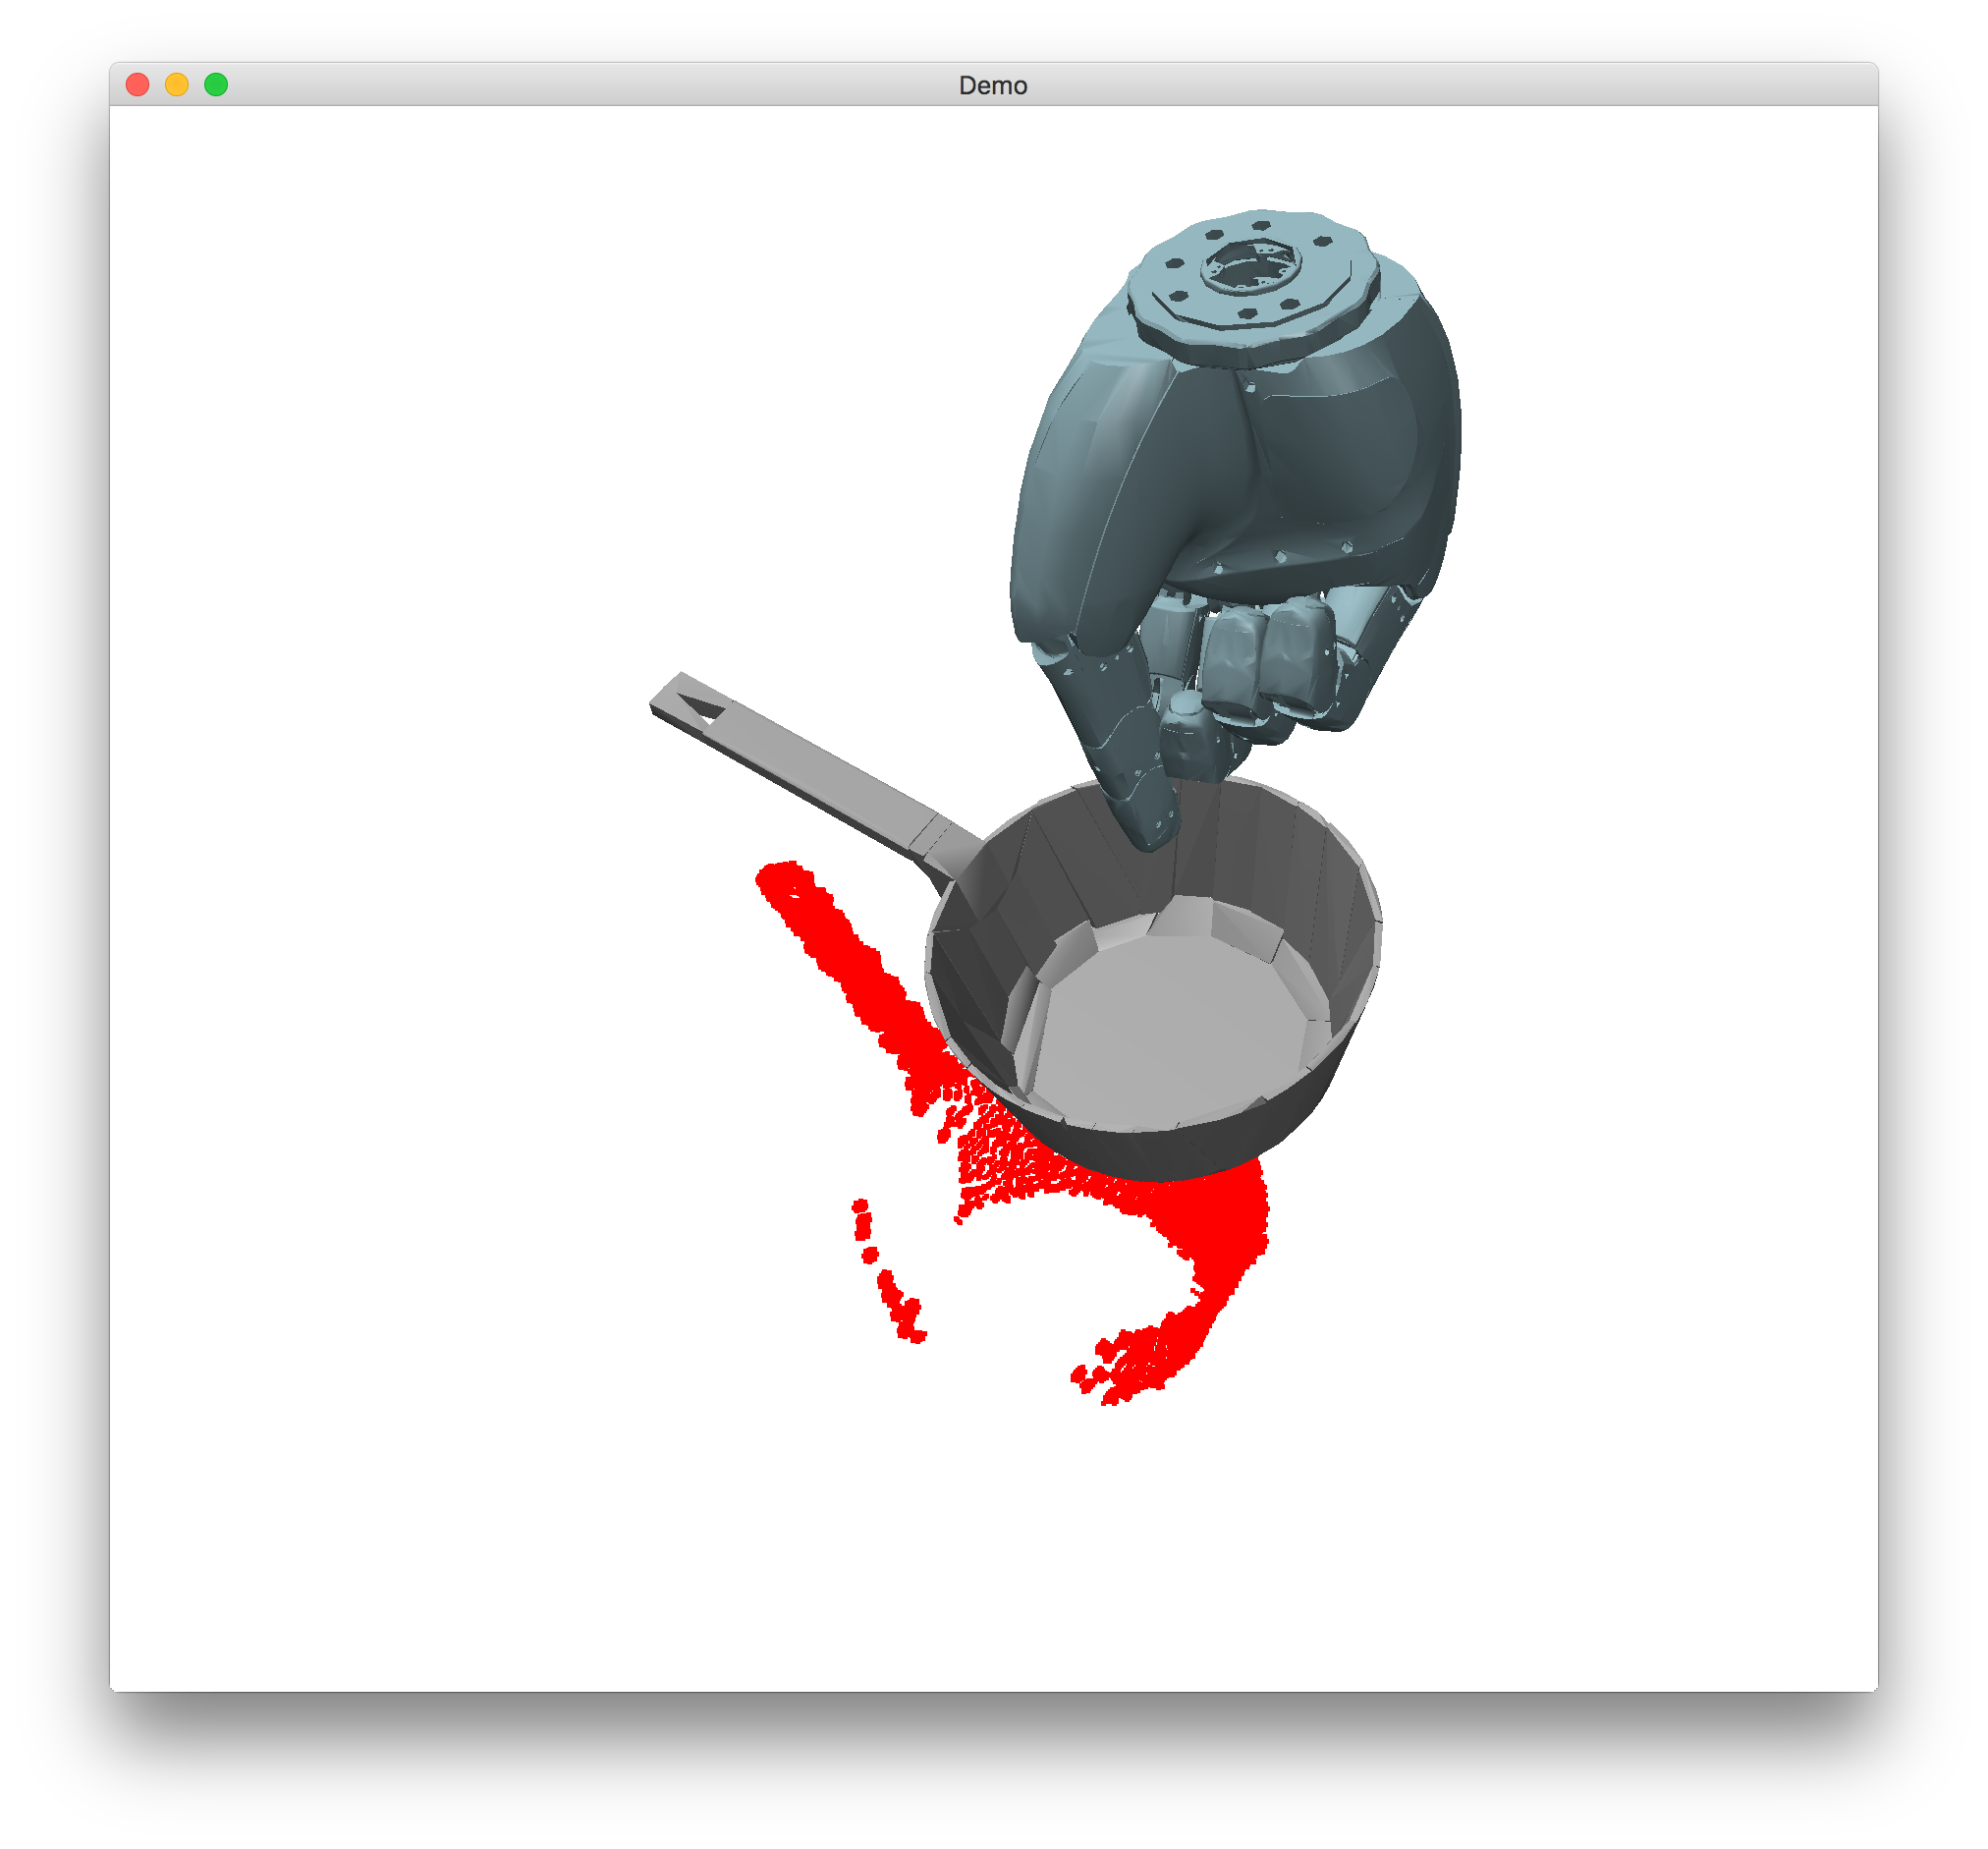
\includegraphics[width=0.24\textwidth]{images/Pan4_2_LFLW}
%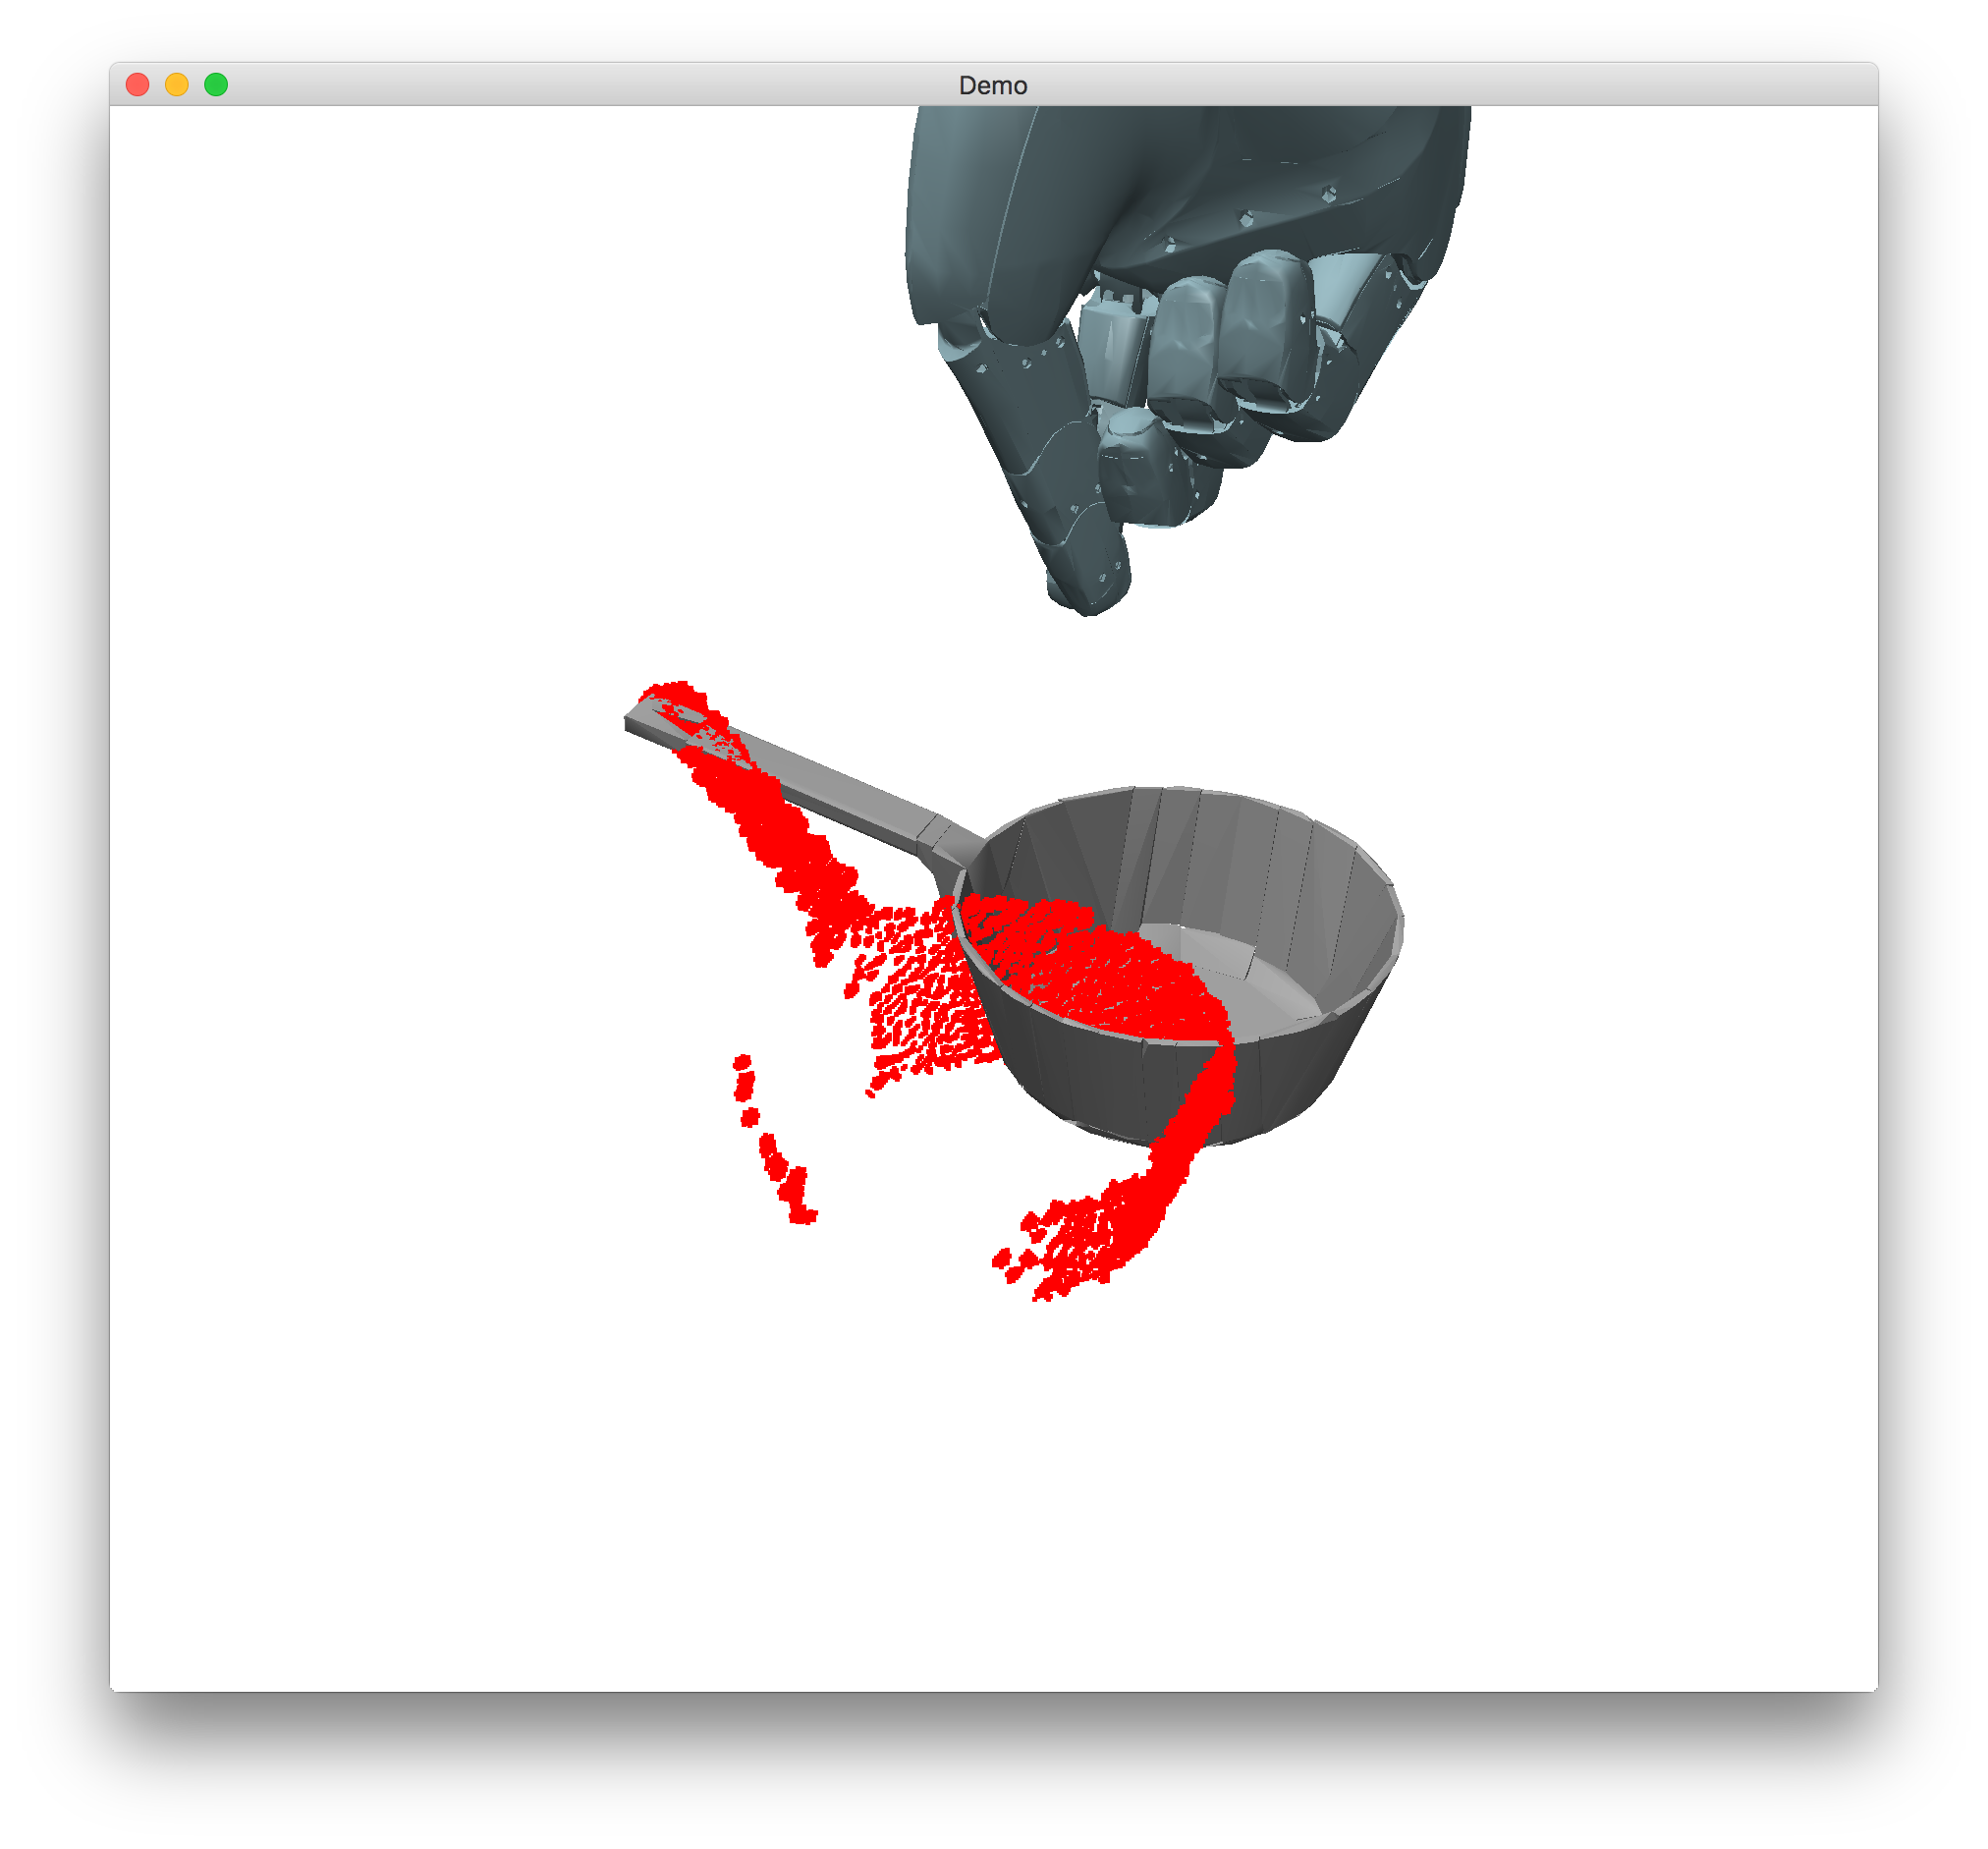
\includegraphics[width=0.24\textwidth]{images/Pan4_2_HFHW}
%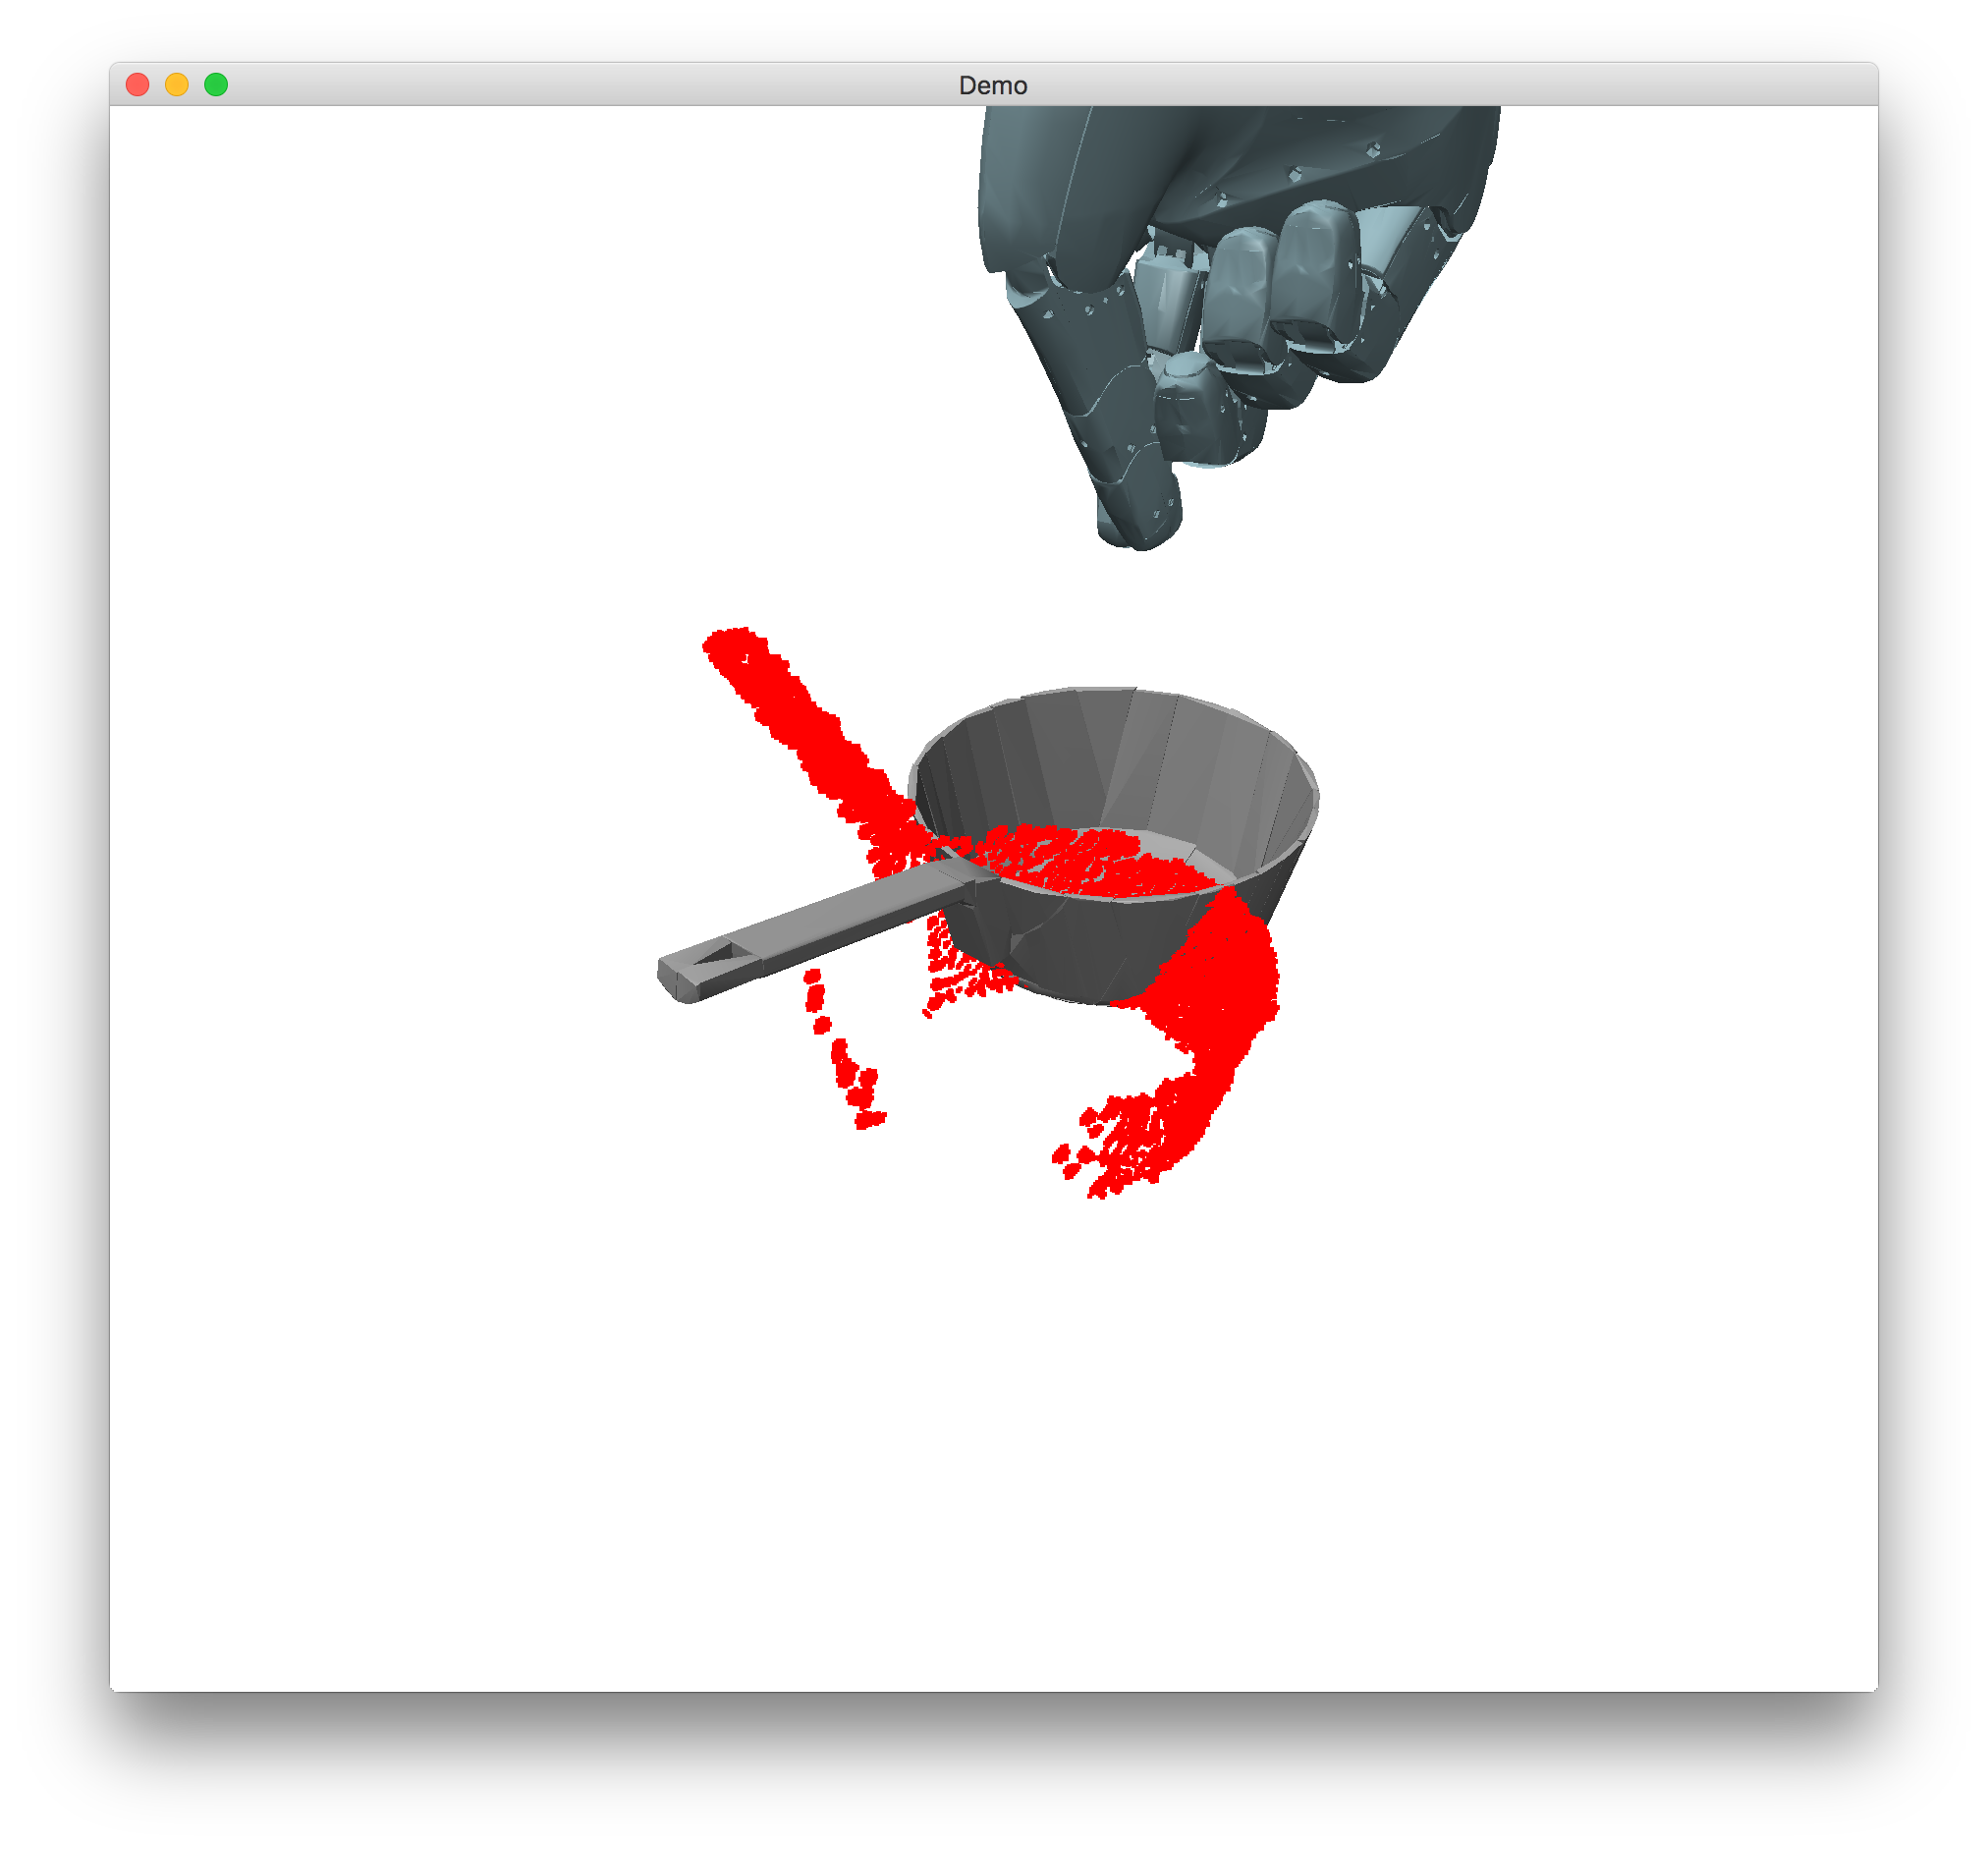
\includegraphics[width=0.24\textwidth]{images/Pan4_2_LFHW}\\
%%
\includegraphics[width=0.96\textwidth]{images/key-to-eval-training}\\
%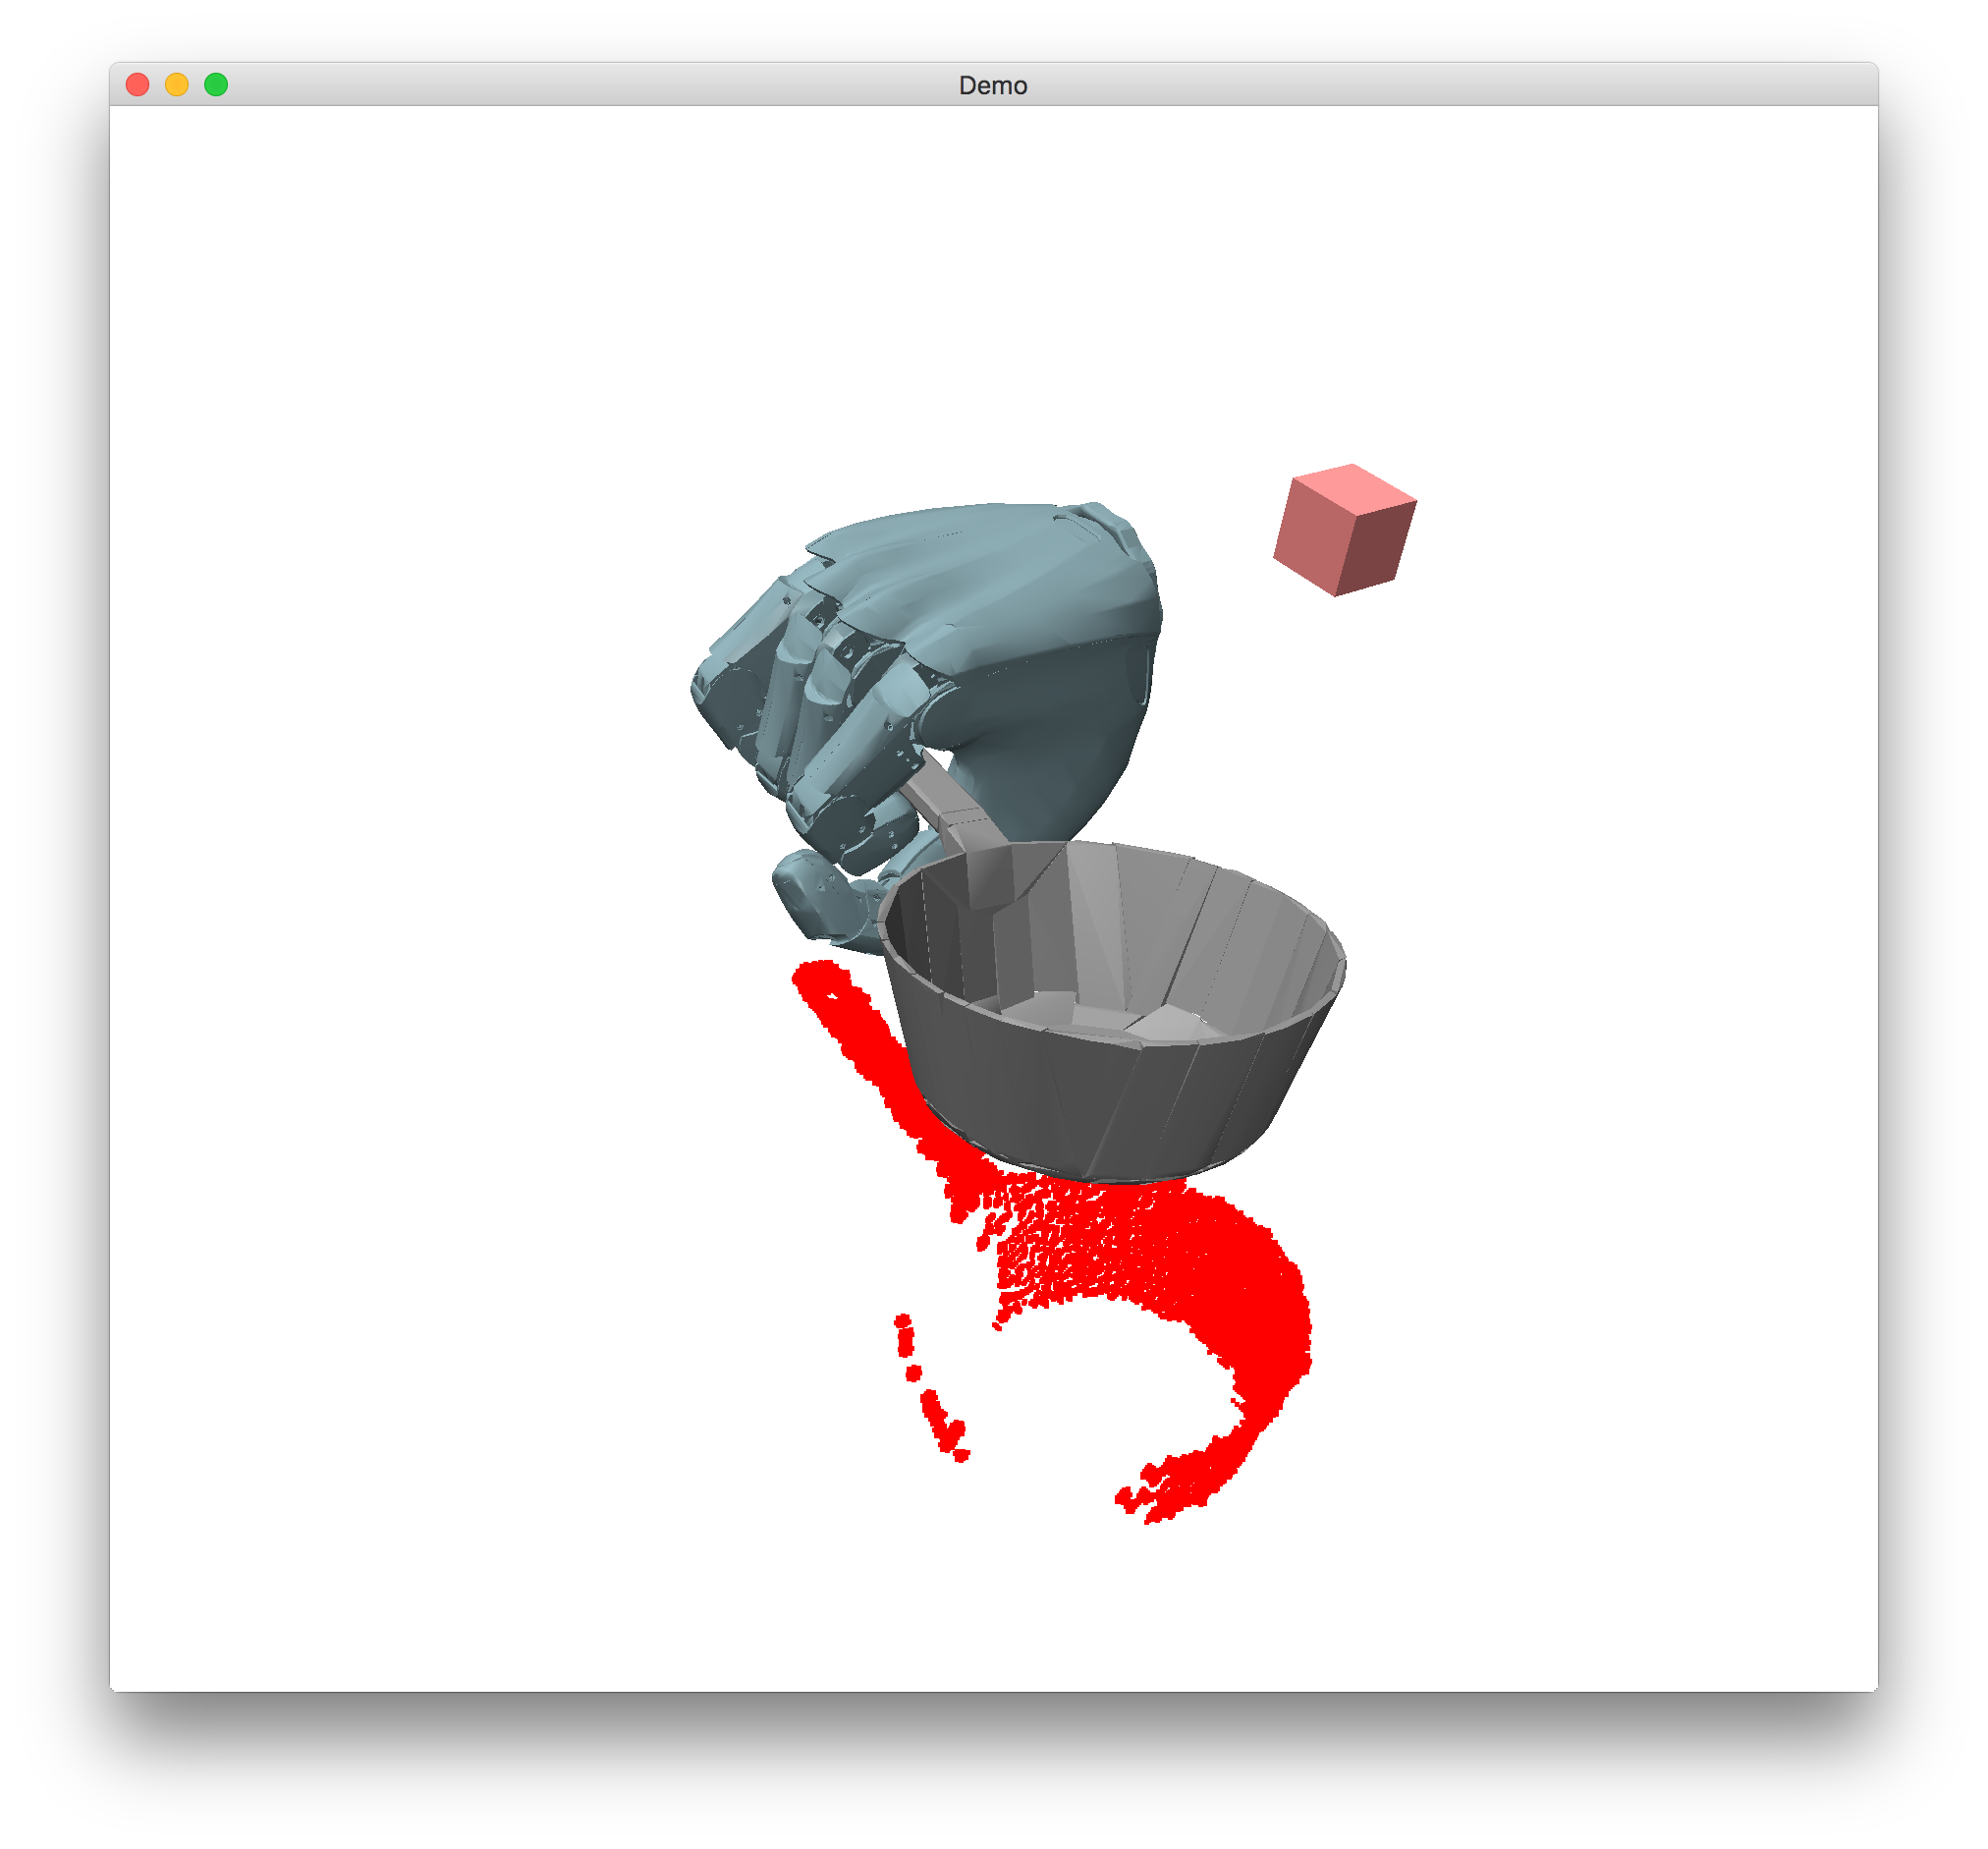
\includegraphics[width=0.24\textwidth]{images/Pan4_HFLW}
%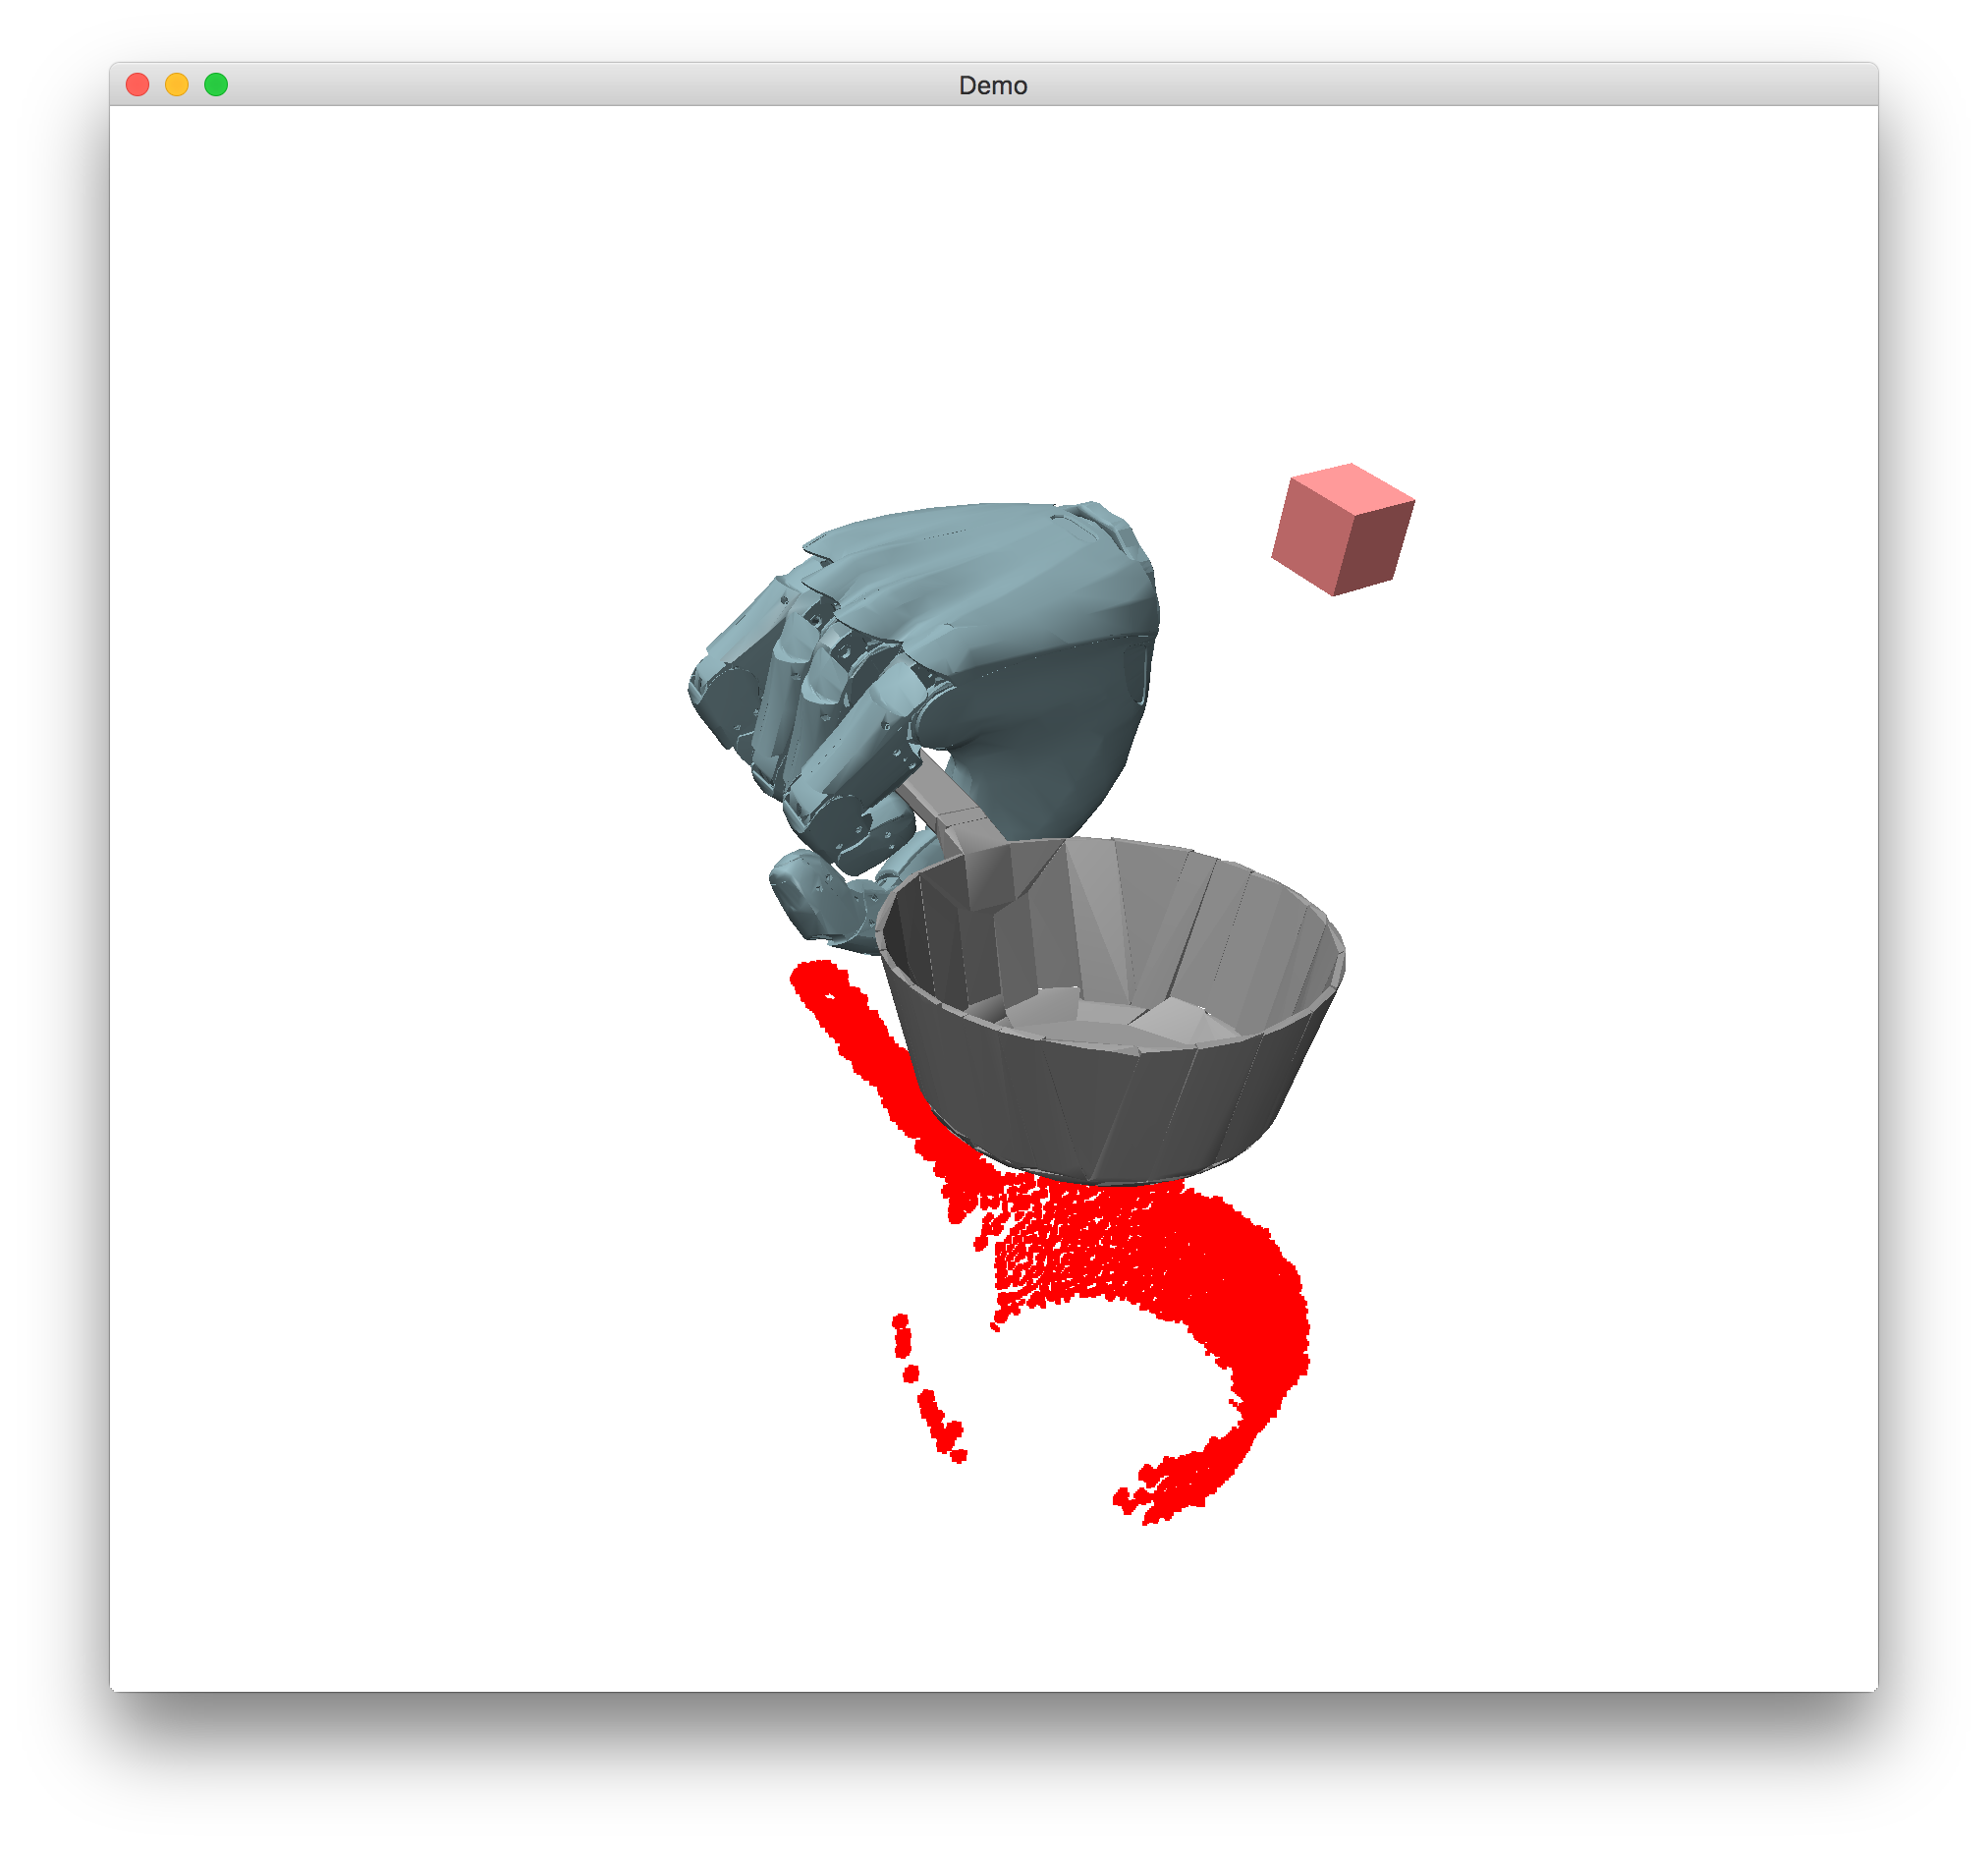
\includegraphics[width=0.24\textwidth]{images/Pan4_LFLW}
%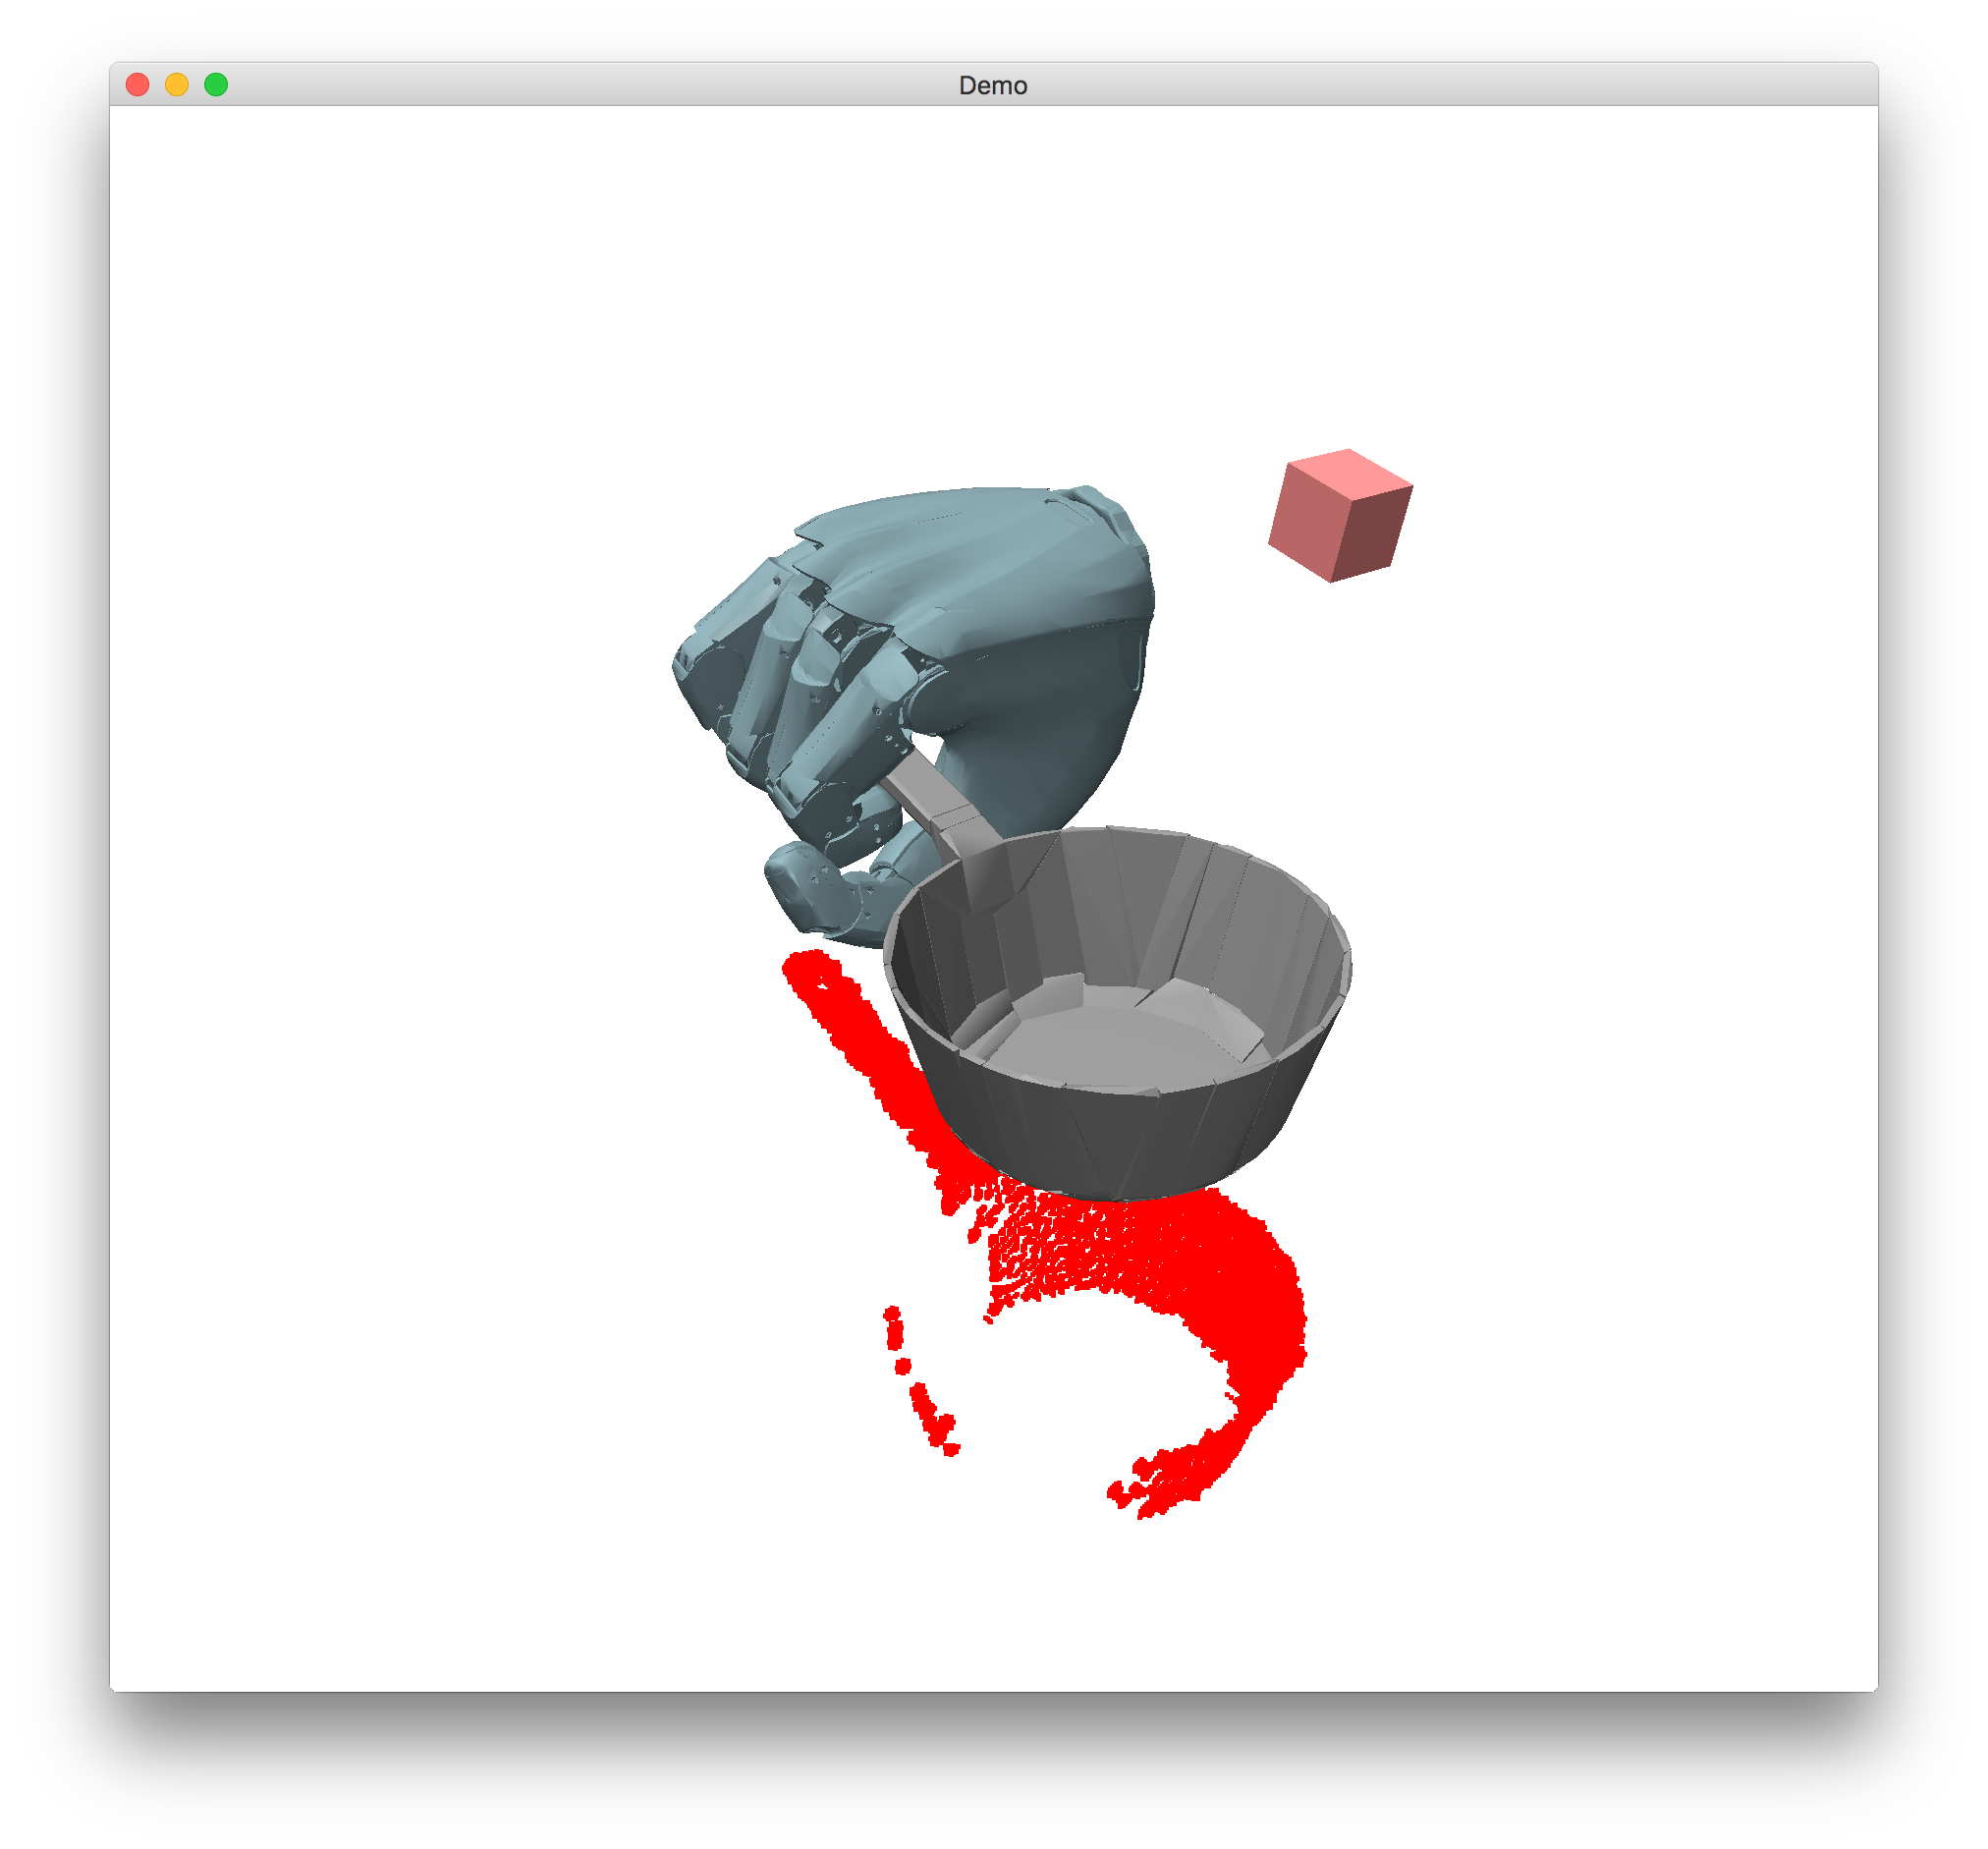
\includegraphics[width=0.24\textwidth]{images/Pan4_HFHW}
%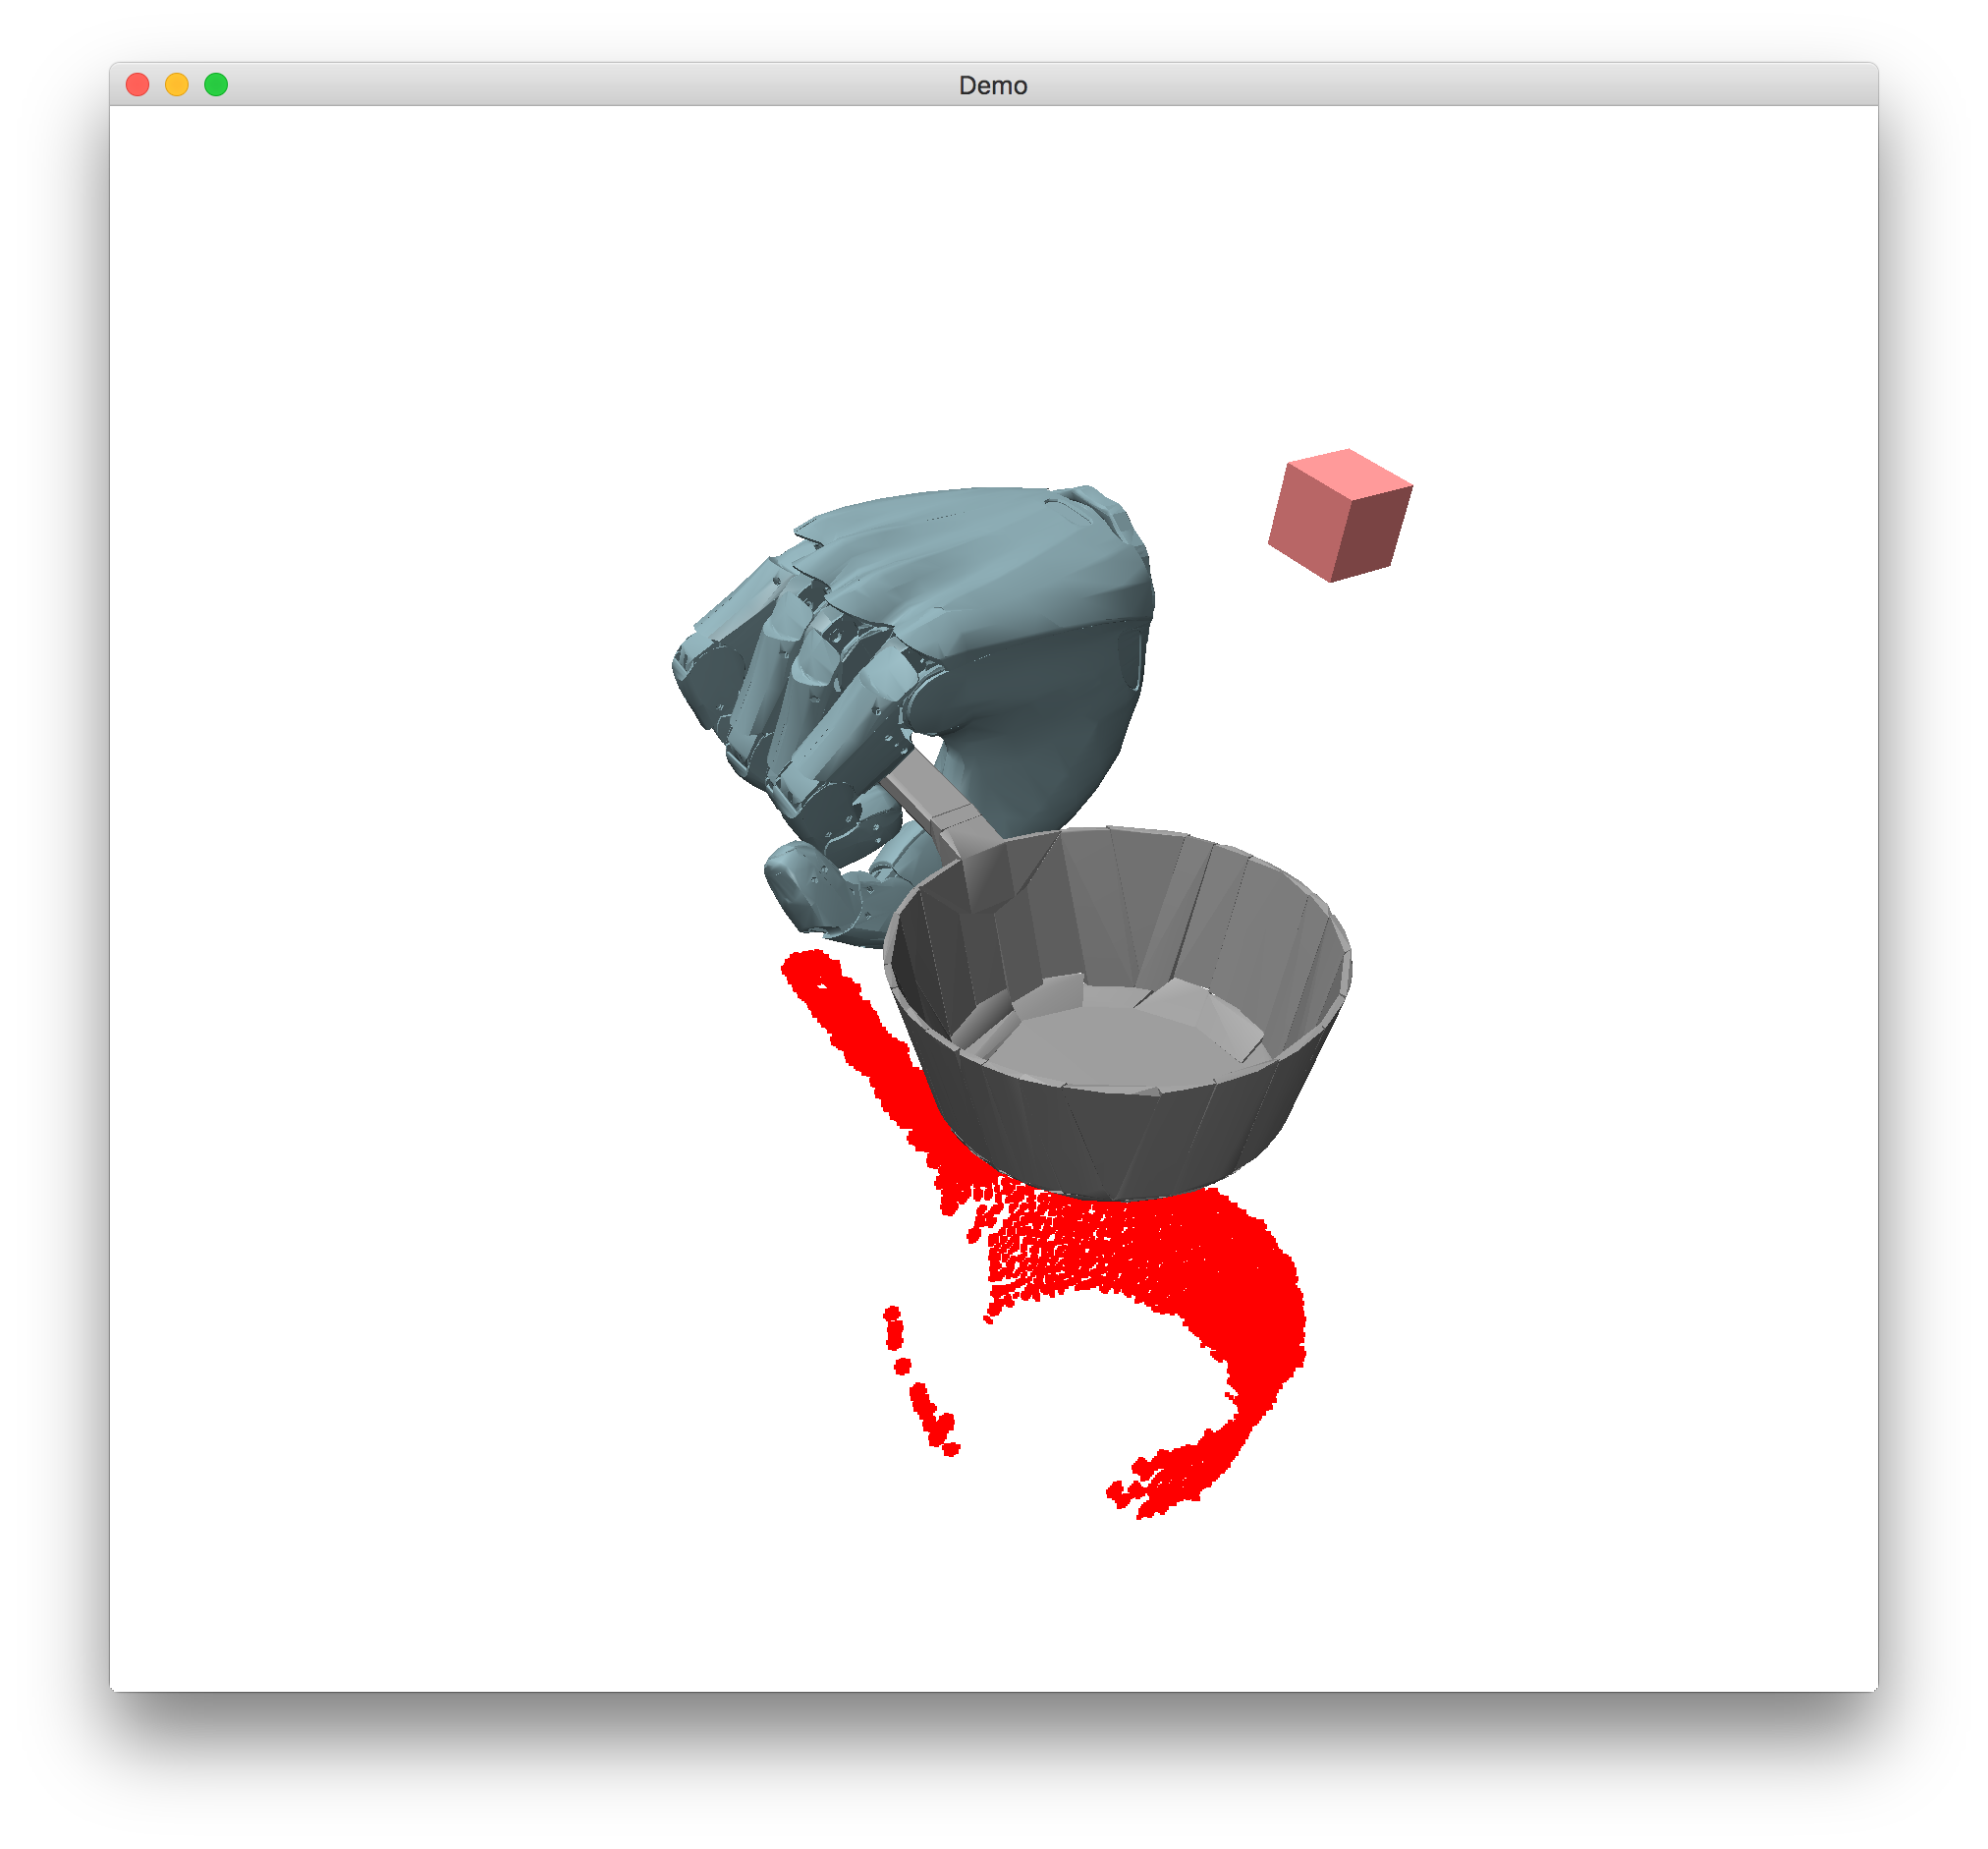
\includegraphics[width=0.24\textwidth]{images/Pan4_LFHW}
\caption{Creating a data set for robust evaluation. (Top row) The same pinch grasp, executed on the same object, with varying friction and mass parameters. (Bottom row) A more robust power grasp, executed on the same object, with the same variation in friction and mass. \label{fig:evaluative-training}}
\end{figure}

Using this method, we generated a data set (DS1) of 1.28 million simulated grasps using GM1 as the generative model and a data set of 1.136 million additional grasps (DS2) using GM2 \footnote{Visit \href{https://rusen.github.io/DDG/}{this website} to download the data.}. Each grasp in DS1-test and DS2 can be replayed in MuJoCo and the sets are decomposed for train, validation and test purposes. We give details of the statistics in Table~\ref{tab:data} including the way that we break down the data-set into training, validation and test subsets. The ratio of successful grasps in the dataset is less than 50\% for GM1, and is more than 50\% for GM2. In order to have a balanced training set, DS1 and DS2 only contain scenes that have at least one successful grasp. During training, the number of successful and unsuccessful grasps have been equalised by under-sampling the failure cases in DS1 and over-sampling the failure cases for DS2. No balancing was performed for the validation and test sets.
\begin{table*}[t]
\centering
\caption{Statistics of the simulated data sets.}
\label{tab:data}
\begin{tabular}{|l|l|l|l|l|l|l|l|l|l|l|} \hline
Data set & Generative &  Subset & \# Scenes & Top-grasp & Top-grasp & Top grasp & Total & Total  & Total  & Total \\ 
              & Model         &              &                   &  \# succs  & \# fails       & \% succs  & grasps   & \# succs      & \# fails  & \% succs  \\ \hline
 DS1-Tr & GM1 & Train & 17714 & 10100 & 7614 & 57.0\% & 1,058,430 & 479,941 & 578,489 & 45.3\% \\ \hline
 DS1-V  & GM1 & Validate & 2309 & 1290 & 1019 & 55.9\% & 122,944 & 61,256 & 61,688 & 49,8\% \\ \hline
 DS1-Te & GM1& Test & 1539 & 1070 & 469 & 69.5\% & 99,521 & 48,084 & 51,437 & 48.3\% \\ \hline
 DS2-Tr  & GM2 & Train & 5377 & 3771 & 1606 & 70.1\% & 943,481 & 533,282 & 410,199 & 56.5\% \\ \hline
 DS2-V   & GM2 & Validate & 544 & 378 & 166 & 69.4\% & 68,586 & 39,559 & 29,027 & 57.7\% \\ \hline
 DS2-Te  & GM2 & Test & 988 & 781 & 207 & 79.0\% & 124,137 & 73,836 & 50,301 & 59.5\% \\ \hline
\end{tabular}
\end{table*}